\chapter{Event Selection}\label{cha:event_selection}

The \Httllfull{} decay has a detector signature of exactly two light leptons ($e$ or $\mu$) of opposite electric
charge and some amount of missing transverse energy due to the neutrinos.
The lepton combinations can be either two electrons ($\epem$), two muons ($\mpmm$), or one electron and on muon ($e^\pm \mu^\mp$).
The decay channels are labeled as $ee$ and $\mu\mu$ for same flavour (SF) combinations and $e\mu$ or $\mu e$ for
different flavour (DF) combinations.
The leptons and jets are each arranged according to their transverse momentum in descending order.
They are labeled with integer numbers, starting with $1$.
The lepton or jet with the highest transverse momentum is called \emph{leading},
the next one is denoted as \emph{subleading}.
If a quantity uses both leading and subleading lepton or jet, it will be indicated by a $\ell\ell$ or jj label, respectively.

This chapter gives an overview of the selection criteria applied to select signal candidate events.
The requirements are applied to both data and simulation.
Since the mass reconstruction in the \Httllfull{} decay channel is non-trivial due to the multiple neutrinos,
advanced mass reconstruction methods are introduced in \cref{sec:event_selection:mass}.
Triggers (\cref{sec:event_selection:trigger}) are used to select events with two final state leptons.
After a common preselection (\cref{sec:event_selection:preselection}) further selection criteria are applied
to select events which fall in the VBF and boosted topology (\cref{sec:event_selection:categorization}).
This allows to separate the Higgs bosons which are produced via the VBF and ggF mechanism.

The selection introduced in this chapter will be referred to as cut-based analysis (CBA) to differentiate
between the multivariate analysis (MVA) as discussed in \cref{cha:mva}, which has a slightly different event selection.

\section{Invariant mass reconstruction}\label{sec:event_selection:mass}

The invariant mass of the Higgs boson candidates (i.e.\ the invariant mass of the di-$\tau$ system)
cannot be calculated without ambiguity since there are four neutrinos in the final state of the $\Httll$ decay.
Since the di-$\tau$ mass can be used to discriminate between signal and background processes and enables
a direct measurement of the mass of the Higgs boson a, correct and precise reconstruction is needed.
In the next sections two approaches are introduced, the collinear approximation and the missing mass calculator.

\subsection{Collinear approximation}\label{sub:event_selection:mcoll}

For the collinear approximation~\cite{MCollAssumption,MColl} it is assumed that the $\etmiss$ originates only
from the $\Htt$ decay and that each $\tau$-lepton is emitted in the same direction as its corresponding visible decay
product (the lepton).
The second assumption is called collinearity.
This is a valid assumption, since $m_H / 2 \gg m_\tau$, which leads to highly boosted taus.

With those two assumptions the invariant mass $\mcoll$ of the di-$\tau$ system can be calculated with
\begin{equation}
    \label{eq:mcoll}
    \mcoll = \frac{\mll}{\sqrt{x_1 x_2}} \,,
\end{equation}
where $\mll$ is the mass of the dilepton system, which is constituted of the visible decay products of the
$\tau$-lepton decay.
The momentum fraction which each visible decay product holds in comparison to the decaying $\tau$-lepton
is denoted as $x_{1,2}$,
\begin{equation}
    \label{eq:mcoll:xdef}
    \pt^{\ell_i} = x_i \pt^{\tau_i} \,, \qquad i = 1,2 \,.
\end{equation}
It can be calculated with
\begin{equation}
    \label{eq:mcoll:xcalc}
    x_{1,2} = \frac{p_x^{\ell_1} p_y^{\ell_2} - p_y^{\ell_1} p_x^{\ell_2}}{p_x^{\ell_1} p_y^{\ell_2} \pm \etmissx p_y^{\ell_{2,1}} - p_y^{\ell_1} p_x^{\ell_2} \mp \etmissy p_x^{\ell_{2,1}}} \,.
\end{equation}

The collinear approximation works well when the di-$\tau$ system is boosted and the approximations are valid.
However, if the two taus are back-to-back ($\Delta \eta (\tau_1,\tau_2) = \pi$), the missing transverse energy
due to the neutrinos cancels partially and the equation system which results in \cref{eq:mcoll:xcalc} cannot
be solved anymore.
This can be prevented by a requirement on the $\eta$ difference of the visible decay products, \detall, or a direct
cut on the momentum fractions, which discards events with unphysical solutions ($x < 0$ or $x > 1$).

\subsection{Missing mass calculator}\label{sub:event_selection:mmc}

If the assumption of collinearity of the decay products of the $\tau$-leptons is not made, there
is no unique solution for the invariant mass of the di-$\tau$ system.
By using on-shell conditions for the $\tau$-lepton masses and the formula to calculate the
missing transverse energy (assuming that all \etmiss{} originates from the $ \tau$-lepton decays),
the following set of equations can be constructed.

\begin{equation}
    \label{eq:mmc:equations}
    \begin{aligned}
        \etmissx &= p^{\text{miss}_1} \sin \theta_{\text{miss}_1} \cos \phi_{\text{miss}_1} + p^{\text{miss}_2} \sin \theta_{\text{miss}_2} \cos \phi_{\text{miss}_2} \\
        \etmissy &= p^{\text{miss}_1} \sin \theta_{\text{miss}_1} \sin \phi_{\text{miss}_1} + p^{\text{miss}_2} \sin \theta_{\text{miss}_2} \sin \phi_{\text{miss}_2} \\
        m_{\tau_1}^2 &= m_{\text{miss}_1}^2 + m_{\ell_1}^2 + 2 \sqrt{p^{\ell_1} + m_{\ell_1}^2} \sqrt{p^{\text{miss}_1} + m_{\text{miss}_1}^2} \\ 
                     & \quad - 2 p^{\ell_1} p^{\text{miss}_1} \cos{(\theta_{\ell_1} - \theta_{\text{miss}_1})} \\
        m_{\tau_2}^2 &= m_{\text{miss}_2}^2 + m_{\ell_2}^2 + 2 \sqrt{p^{\ell_2} + m_{\ell_2}^2} \sqrt{p^{\text{miss}_2} + m_{\text{miss}_2}^2}\\
                     & \quad - 2 p^{\ell_2} p^{\text{miss}_2} \cos{(\theta_{\ell_2} - \theta_{\text{miss}_2})}
    \end{aligned}
\end{equation}

The known variables are the components of the missing transverse energy ($\etmissx$ and $\etmissy$)
and the momenta and invariant masses of the visible decay products of the $\tau$-leptons ($\ell_1$ and $\ell_2$).
Unknown are the momenta, masses, and angles ($\phi$ and $\theta$) of the two neutrino systems, which are composed of two neutrinos each.
These quantities are labeled with $\text{miss}_1$ and $\text{miss}_2$.

Since this system of equations is underconstrained there is no single solution.
However, the different solutions have different probabilities to occur due to the matrix element of the $\tau$-decay.
The missing mass calculator (MMC) algorithm~\cite{MMC} scans over four of the unknown variables ($m_{\text{miss}_{1,2}}$ and $\Phi_{\text{miss}_{1,2}}$),
solves the system of equations and assigns each solution the corresponding probability obtained by calculating the matrix
element of the $\tau$-decay with the solution-specific kinematics.
The resolution of the $\etmissx$ and $\etmissy$ variables is also included in the scan, because the MMC algorithm
is affected by the resolution of $\etmiss$.
The algorithm can fail to converge if the $\etmiss$ is badly reconstructed.
To obtain only one solution either the most probable solution can be chosen or an average over all solutions,
weighted by the corresponding probability, can be calculated.
In this analysis the former approach is chosen.


\section{Trigger}\label{sec:event_selection:trigger}

Triggers are used to select events with two leptons ($ee$, $e\mu$\footnote{In this section $e\mu$ indicates all events
with one electron and one muon, the differentiation between $e\mu$ and $\mu e$ is not made here.}, $\mu\mu$) in the final state.
A general overview of the ATLAS trigger system was given in \cref{sub:setup:trigger}.
Both single-lepton and dilepton triggers are used.
They differ between the 2015 and 2016 data taking period due to the increase in luminosity.

\begin{table}[htpb]
    \centering
    \caption{Single-lepton triggers and offline $\pt$ thresholds for the 2015 and 2016 data set used in the $\Httll$ analysis.}\label{tab:event_selection:trigger:single}
    \begin{tabular}{@{}llll@{}}
        \toprule
        Lepton flavour & Year & Trigger & Threshold \\ \midrule
        Electron       & 2015 & \texttt{HLT\_e24\_lhmedium\_L1EM20VH} & \multirow{3}{*}{$\pt > \unit[25]{GeV}$} \\
                       &      & \texttt{HLT\_e60\_lhmedium} \\
                       &      & \texttt{HLT\_e120\_lhloose} \\ \cmidrule(l){2-4}
                       & 2016 & \texttt{HLT\_e26\_lhtight\_nod0\_ivarloose} & \multirow{3}{*}{$\pt > \unit[27]{GeV}$} \\
                       &      & \texttt{HLT\_e60\_lhmedium\_nod0} \\
                       &      & \texttt{HLT\_e140\_lhloose\_nod0} \\ \midrule
        Muon           & 2015 & \texttt{HLT\_mu20\_iloose\_L1MU15} & \multirow{2}{*}{$\pt > \unit[21]{GeV}$} \\
                       &      & \texttt{HLT\_mu50} \\ \cmidrule(l){2-4}
                       & 2016 & \texttt{HLT\_mu26\_ivarmedium} & \multirow{2}{*}{$\pt > \unit[28]{GeV}$} \\
                       &      & \texttt{HLT\_mu50} \\
        \bottomrule
    \end{tabular}
\end{table}

\begin{table}[htpb]
    \centering
    \caption{Dilepton triggers offline $\pt$ thresholds for the 2015 and 2016 data set used in the $\Httll$ analysis.}\label{tab:event_selection:trigger:di}
    \begin{tabular}{@{}llll@{}}
        \toprule
        Channel  & Year & Trigger & Threshold \\ \midrule
        $ee$     & 2015 & \texttt{HLT\_2e12\_lhloose\_L12EM10VH} & $\pt^{e_1, e_2} > \unit[15]{GeV}$ \\
                 & 2016 & \texttt{HLT\_2e17\_lhvloose\_nod0} & $\pt^{e_1, e_2} > \unit[18]{GeV}$ \\ \cmidrule{1-4}
        $e\mu$   & 2015 & \texttt{HLT\_e17\_loose\_mu14} & $\pt^{e} > \unit[18]{GeV}, \pt^\mu > \unit[15]{GeV}$ \\
                 & 2016 & \texttt{HLT\_e17\_lhloose\_nod0\_mu14} & $\pt^{e} > \unit[18]{GeV}, \pt^\mu > \unit[15]{GeV}$ \\ \cmidrule{1-4}
        $\mu\mu$ & 2015 & \texttt{HLT\_mu18\_mu8noL1} & $\pt^{\mu_1} > \unit[19]{GeV}, \pt^{\mu_2} > \unit[10]{GeV}$ \\
                 & 2016 & \texttt{HLT\_mu22\_mu8noL1} & $\pt^{\mu_1} > \unit[24]{GeV}, \pt^{\mu_2} > \unit[9]{GeV}$ \\
        \bottomrule
    \end{tabular}
\end{table}

The triggers for the $\Httll$ analysis are listed in \cref{tab:event_selection:trigger:single,tab:event_selection:trigger:di}.
Multiple triggers for the same object and data taking period are combined with a logical `or'.
The overlap of single-lepton and dilepton triggers is avoided to prevent difficulties with the trigger efficiencies
by selecting the triggers based on the transverse momentum of the lepton.
Lower $\pt$ thresholds are used for dilepton triggers and higher ones for single-lepton triggers as
illustrated in \cref{fig:event_selection:triggers}.

\begin{figure}[htpb]
    \centering
        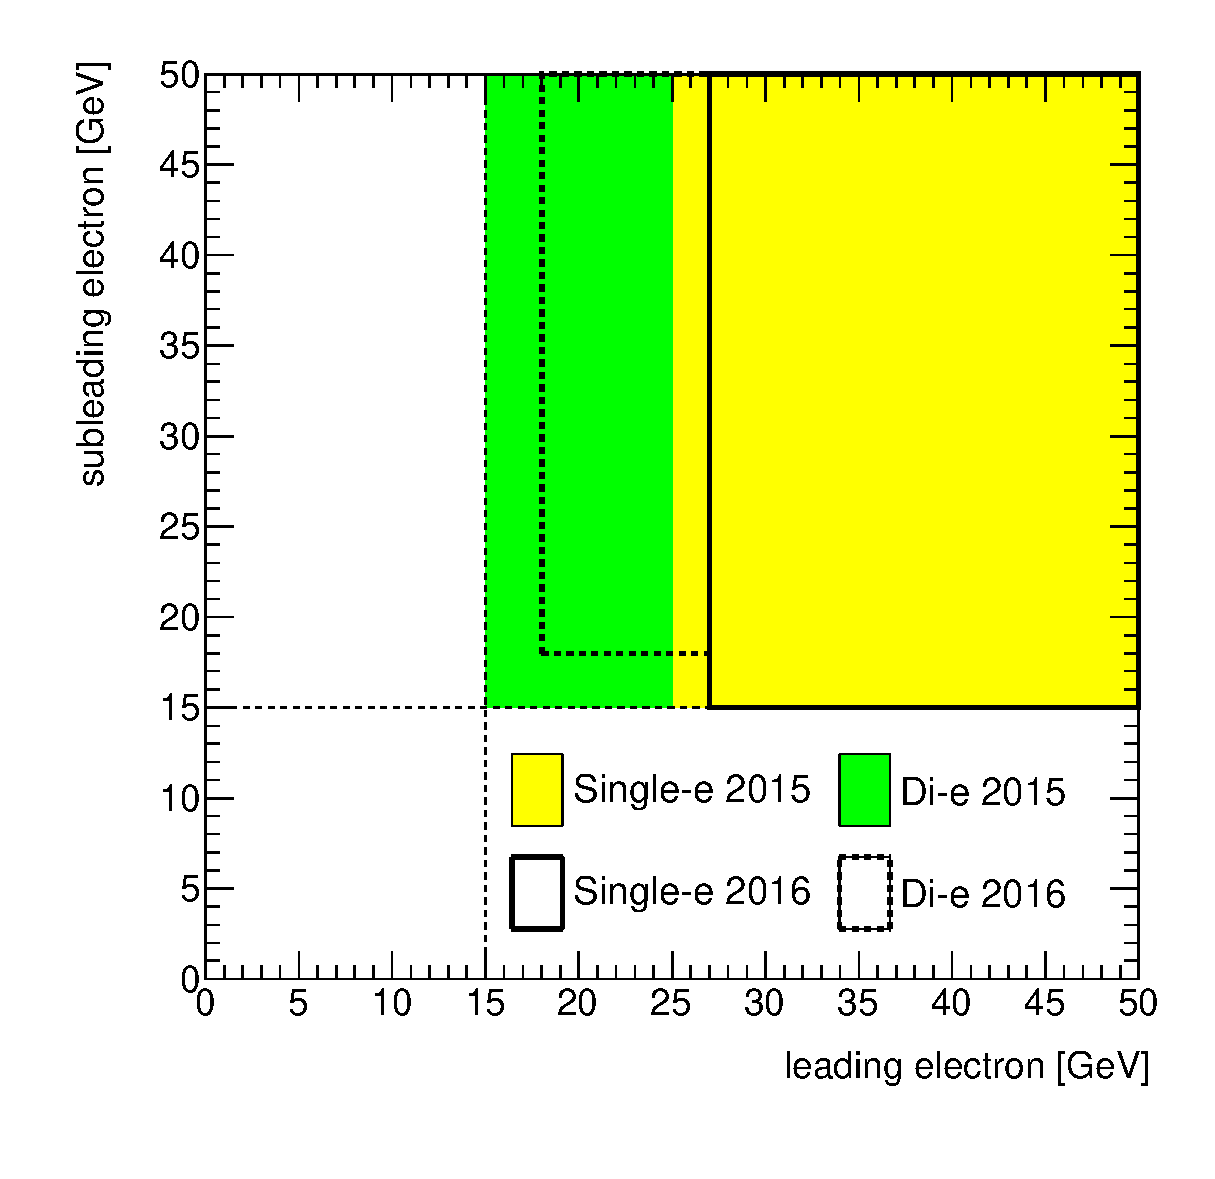
\includegraphics[width=0.3\textwidth]{./figures/event_selection/triggers_ee.eps}
        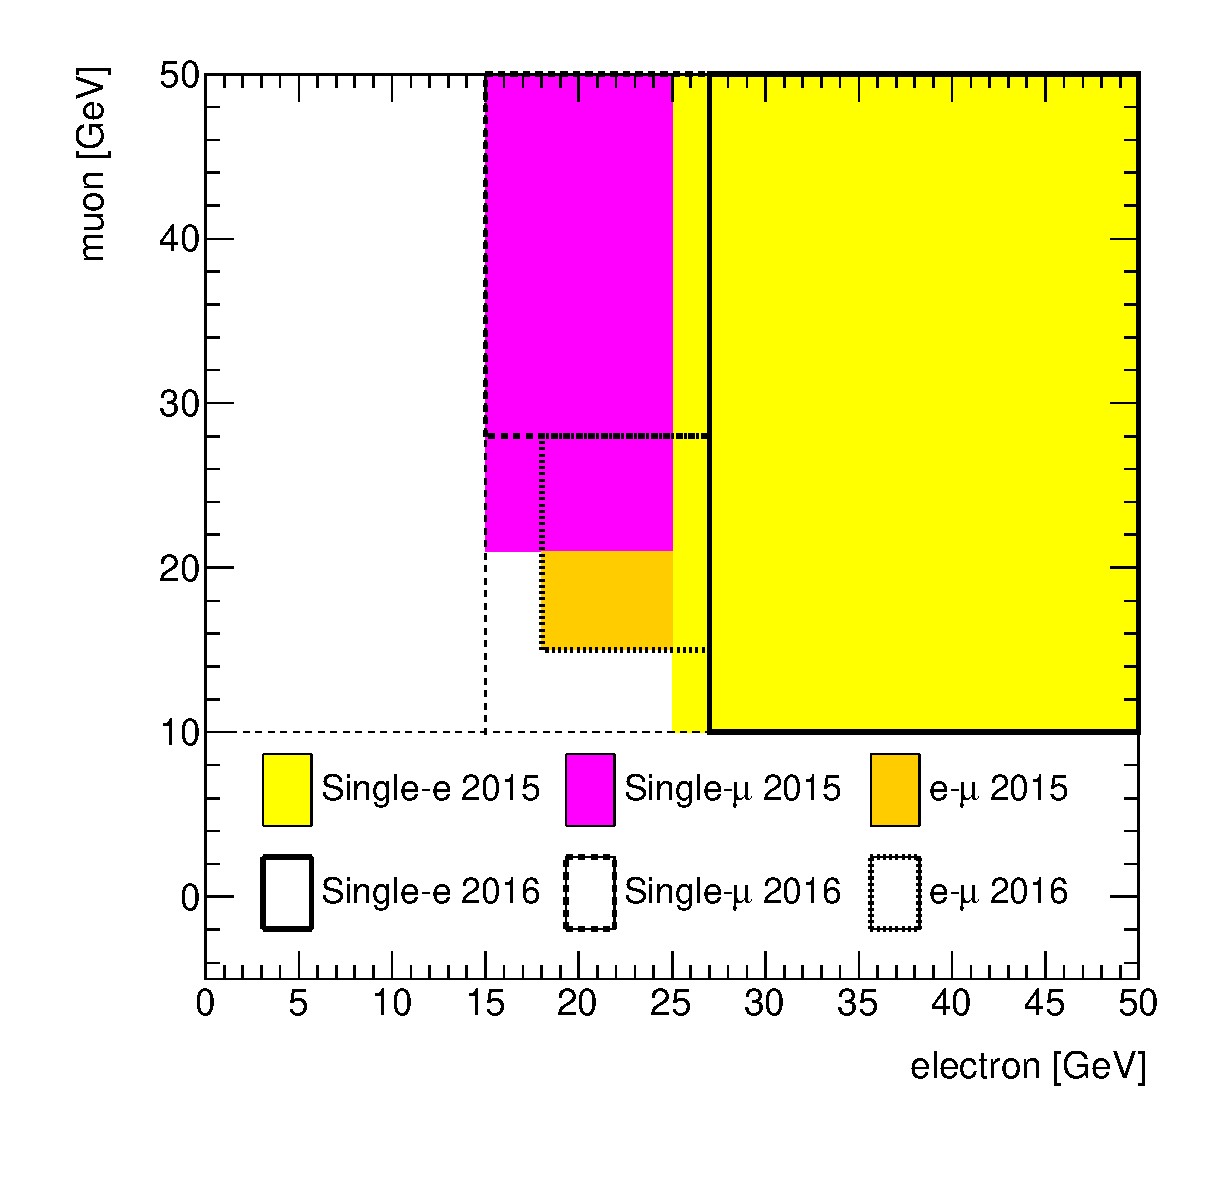
\includegraphics[width=0.3\textwidth]{./figures/event_selection/triggers_emu.eps}
        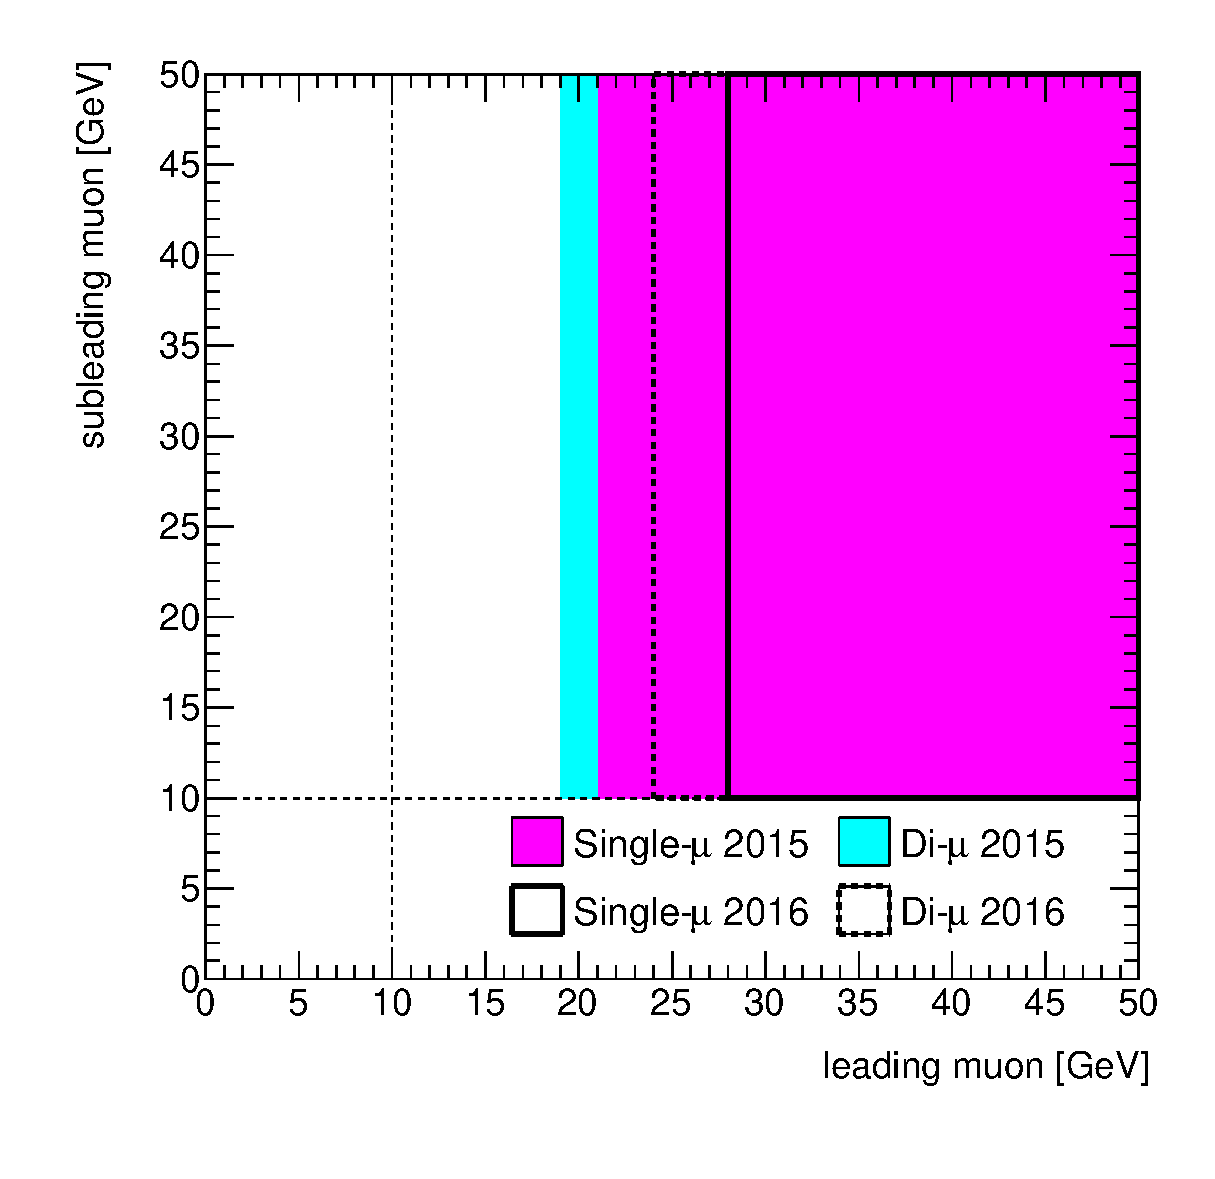
\includegraphics[width=0.3\textwidth]{./figures/event_selection/triggers_mumu.eps}
        \caption{Transverse momentum criteria to select either single-lepton or dilepton triggers in order to avoid overlap.
        The plots correspond to $ee$ (left), $e\mu$ (middle), and $\mu\mu$ (right) final states.~\cite{TauConfNote}}\label{fig:event_selection:triggers}
\end{figure}

Trigger names are composed of a series of acronyms and abbreviations chained together, directly or with underscores,
which define the trigger type and the imposed requirements on the objects to trigger.
For this analysis all trigger names start with \texttt{HLT}, indicating that the software-based High Level Trigger
is used.
Electrons and muons are denoted  as \texttt{e} and \texttt{mu}, respectively, followed by a number defining the transverse
momentum threshold in GeV, which the object has to fulfill.
A preceding number corresponds to multiple objects with the same requirements.
Identification and isolation criteria as introduced in \cref{sec:object_selection:electrons,sec:object_selection:muons}
can be imposed on the triggered objects, which is decoded as \texttt{lhID}
and \texttt{iISO}, where \texttt{ID} and \texttt{ISO} specify the corresponding working points.
If there is no requirement on the distance of the observed tracks to the primary vertex the term \texttt{nod0}
is included.
HLTs can be seeded by L1 triggers, which is indicated by including \texttt{L1} in the trigger name.
L1 trigger names also contain the type of the object to trigger, \texttt{E} and \texttt{M} for electrons and muons, respectively.
Usually, there is a threshold on the missing transverse energy, denoted as \texttt{M} followed by a number,
which corresponds to the threshold in GeV.
The \etmiss{} thresholds can vary slightly as a function of $\eta$, which is denoted with \texttt{V}.
An additional hadronic veto can be applied, which is indicated by \texttt{H}.

To account for differences in the trigger efficiencies correction factors are calculated by comparing
the efficiencies between data and simulation~\cite{Trigger2015,Trigger2016}.
An additional offline $\pt$ requirement is introduced to ensure that the trigger efficiencies are in the plateau region.
The thresholds are $\unit[1-3]{GeV}$ higher than the trigger $\pt$ thresholds.
They can be found in \cref{tab:event_selection:trigger:single,tab:event_selection:trigger:di}.

\section{Preselection}\label{sec:event_selection:preselection}

Before requiring kinematic cuts to purify signal events a series of
requirements to ensure data quality are applied.
\begin{description}[style=nextline,leftmargin=1cm]
    \item[\ \,(1) Good Run List]
        Data events are discarded if they are not included in the good run list,
        which contains the events which were recorded when all sub-detector systems have been in full operational mode.
        This results in an integrated luminosity of $\lumiint = \unit[36.1]{fb^{-1}}$.
    \item[\ \,(2) Primary vertex]
        At least on reconstructed vertex is required, which is consistent with the IP\@.\todo{Additional requirements on the vertex?}\
        This is used to reject events from cosmic rays and beam-halo effects.
    \item[\ \,(3) Jet cleaning and crazy muon veto]
        Events with jet contributions which can not be associated with hard scattering are removed~\cite{JetCleaning2015,JetCleaning2016}. \todo{Crazy muon veto?}
\end{description}
Now basic trigger and preselection cuts are applied to select the decay topology of the \Httll{} decay.
Whenever viable, a distribution of  the signal and different backgrounds is shown for a variable before the cut on
this variable was applied. Normalization factors as defined in \cref{sec:background_estimation:normalization} are applied.
Their values are 1.06 (top), 1.19 (\Zll), and 1.07 (\Ztautau) respectively.
The signal is scaled by factor 20.\todo{Change signal scaling to x50}\
The error bands only contain statistical uncertainties.
\begin{description}[style=nextline,leftmargin=1cm]
    \item[\ \,(4) Number of leptons]
        Exactly two leptons, either two electrons, one electron and on muon, or two muons, with the reconstruction
        and identification criteria defined in \cref{sec:object_selection:electrons,sec:object_selection:muons} are required.
    \item[\ \,(5) Lepton identification and isolation criteria]
        The electrons and muons need to pass the \emph{medium} identification and \emph{gradient} isolation criteria.
    \item[\ \,(6) Hadronic tau veto]
        To ensure orthogonality to the \Httlh{} and \Htthh{} channels all events with one or more hadronic $\tau$-leptons
        obeying the \emph{medium} criterion are vetoed.
    \item[\ \,(7) Trigger]
        The event has to pass on of the triggers as defined in \cref{sec:event_selection:trigger}.
    \item[\ \,(8) Trigger matching]
        The triggered leptons have to match with the reconstructed leptons.
    \item[\ \,(9) Opposite sign] The electric charge of the two leptons has to be opposite.
    \item[(10) Dilepton mass]
        The mass of the dilepton systems is restricted to $\unit[30]{GeV} < \mll < \unit[75\,(100)]{GeV}$ for SF (DF) events.
        This helps to reduce the Drell-Yan $\Zgammall$ background.
        \cref{fig:event_selection:cutflow:mll} shows the $\mll$ distribution for SF and DF events before Cut~10.
    \item[(11) Jet momentum]
        Jets need to have a transverse momentum of $\pt > \unit[25]{GeV}$. At least one jet with $\pt > \unit[40]{GeV}$ is
        required.
        This helps to select both the VBF and boosted category (\cref{sec:event_selection:categorization}).
        The transverse momentum distribution of the leading jet, $\pt^{\text{jet}_1}$, before Cut~11 is shown in \cref{fig:event_selection:cutflow:jetlead}.
    \item[(12) Missing transverse energy]
        For DF events a cut on $\etmiss > \unit[20]{GeV}$ is applied, since neutrinos are expected in the final state.
        To reduce $\Zgammall$ background, the requirement is tightened to $\etmiss > \unit[55]{GeV}$ for SF events.
        \cref{fig:event_selection:cutflow:met} shows the $\etmiss$ distribution for SF and DF events before Cut~12.
    \item[(13) Missing transverse energy (HPTO)]
        The missing transverse energy is calculated from only high-$\pt$ objects (HPTO). Only the two decay leptons and
        all jets with a transverse momentum of $\pt > \unit[30]{GeV}$ are used.
        \begin{equation}
            \label{eq:met:hpto}
            \etmissvecobj{\text{HPTO}} = - \ptvec^{\ell_0} - \ptvec^{\ell_1} - \sum_{\mathclap{\substack{\text{jets} \\ \pt > \unit[30]{GeV}}}} \ptvec^\text{jet}
        \end{equation}
        A HPTO missing transverse energy of $\etmisshpto > \unit[55]{GeV}$ for SF events is required to further reject
        $\Zgammall$ background.
        The \etmisshpto{} distribution is shown for SF events before Cut~13 in \cref{fig:event_selection:cutflow:hpto}.
    \item[(14) Momentum fraction]
        The momentum fractions carried by the visible decay products of the $\tau$-lepton decay are restricted to $0.1 < x_{1,2} < 1.0$.
        They are calculated in the collinear mass approximation (\cref{sub:event_selection:mcoll}).
        This rejects background events where the assumption of collinearity of the $\tau$-lepton and its visible decay product is not valid.
        \cref{fig:event_selection:cutflow:x} shows the distributions of $x_1$ and $x_2$ before Cut~14.
    \item[(15) Angular difference in $\bm{\eta}$]
        This cut limits the $\eta$ difference between the two leptons to $\absdetall < 1.5$.
        The $\absdetall$ distribution before Cut~15 is shown in \cref{fig:event_selection:cutflow:detall}.
    \item[(16) Angular difference in $\bm{\dr}$]
        The $\dr$ separation between the two leptons is required to be $\drll < 2$.
        \cref{fig:event_selection:cutflow:drll} shows the $\drll$ distribution before Cut~16.
    \item[(17) Collinear mass]
        To ensure orthogonality with the $H \to WW$ analysis, the collinear mass (\cref{sub:event_selection:mcoll}) is limited to $\mcoll > m_\Z - \unit[25]{GeV}$.
        The $\mcoll$ distribution before Cut~17 is shown in \cref{fig:event_selection:cutflow:mcoll}.
    \item[(18) MMC mass]
        Events where the MMC mass reconstruction algorithm (\cref{sub:event_selection:mmc}) did not converge are discarded.
    \item[(19) b-jet veto]
        Events which contain $b$-jets (\cref{sec:object_selection:jets}) with $\pt > \unit[25]{GeV}$ are vetoed.
        This helps to reduce the single-top and $\ttbar$ background.
\end{description}

\todo{Some labels of the plots need to be updated to the new indexing scheme. Also the $x_{1,2}$ distributions need a wider range.}

\begin{figure}[htb]
    \centering
    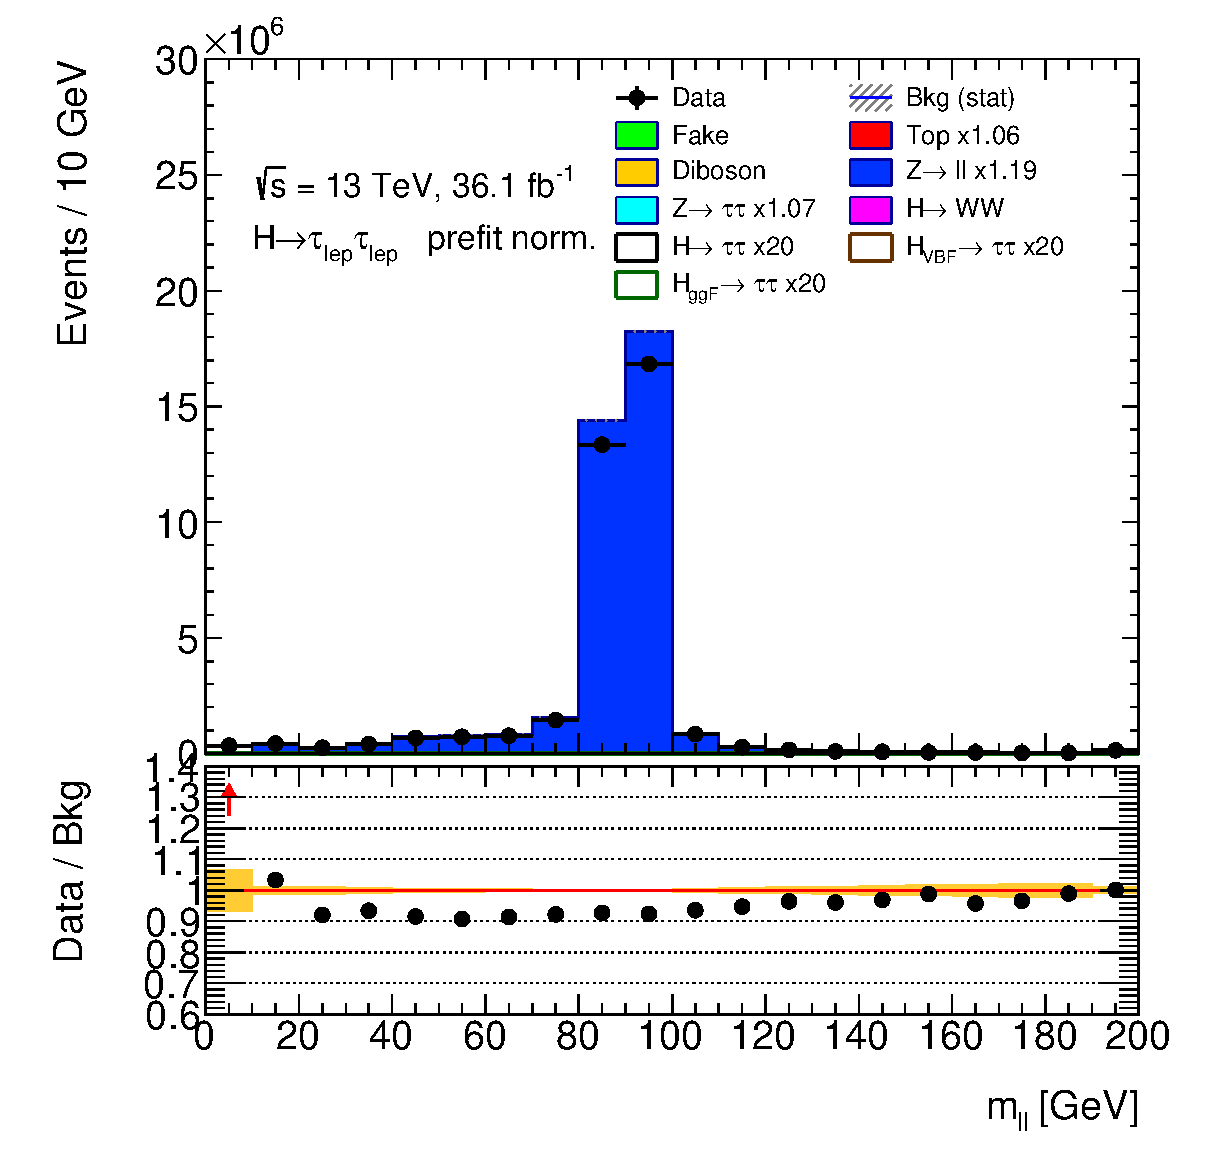
\includegraphics[width=0.45\textwidth]{./plots/event_selection/eemm-CutOS-mvis-lin.eps}
    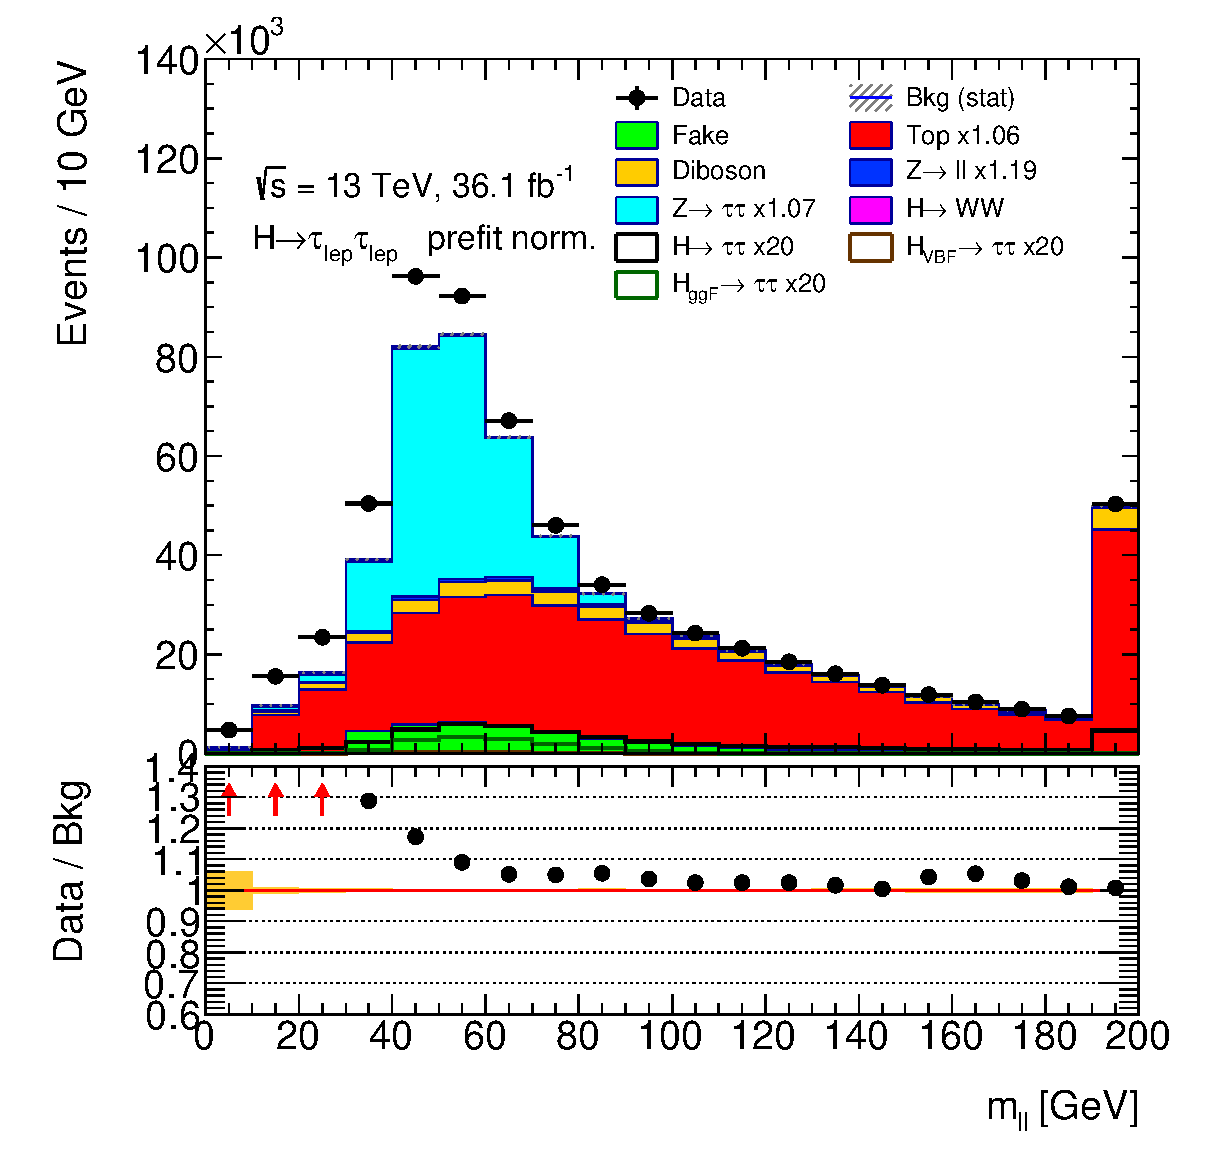
\includegraphics[width=0.45\textwidth]{./plots/event_selection/emme-CutOS-mvis-lin.eps}
    \caption{Distribution of $\mll$ after Cut~9 for SF (left) and DF (right) events.
             Normalization factors are applied on the top-quark, $\Zll$, and $\Ztautau$ background.
             The signal is scaled by a factor of 20.
             Only statistical uncertainties are included in the error band.}\label{fig:event_selection:cutflow:mll}
\end{figure}

\begin{figure}[htb]
    \centering
    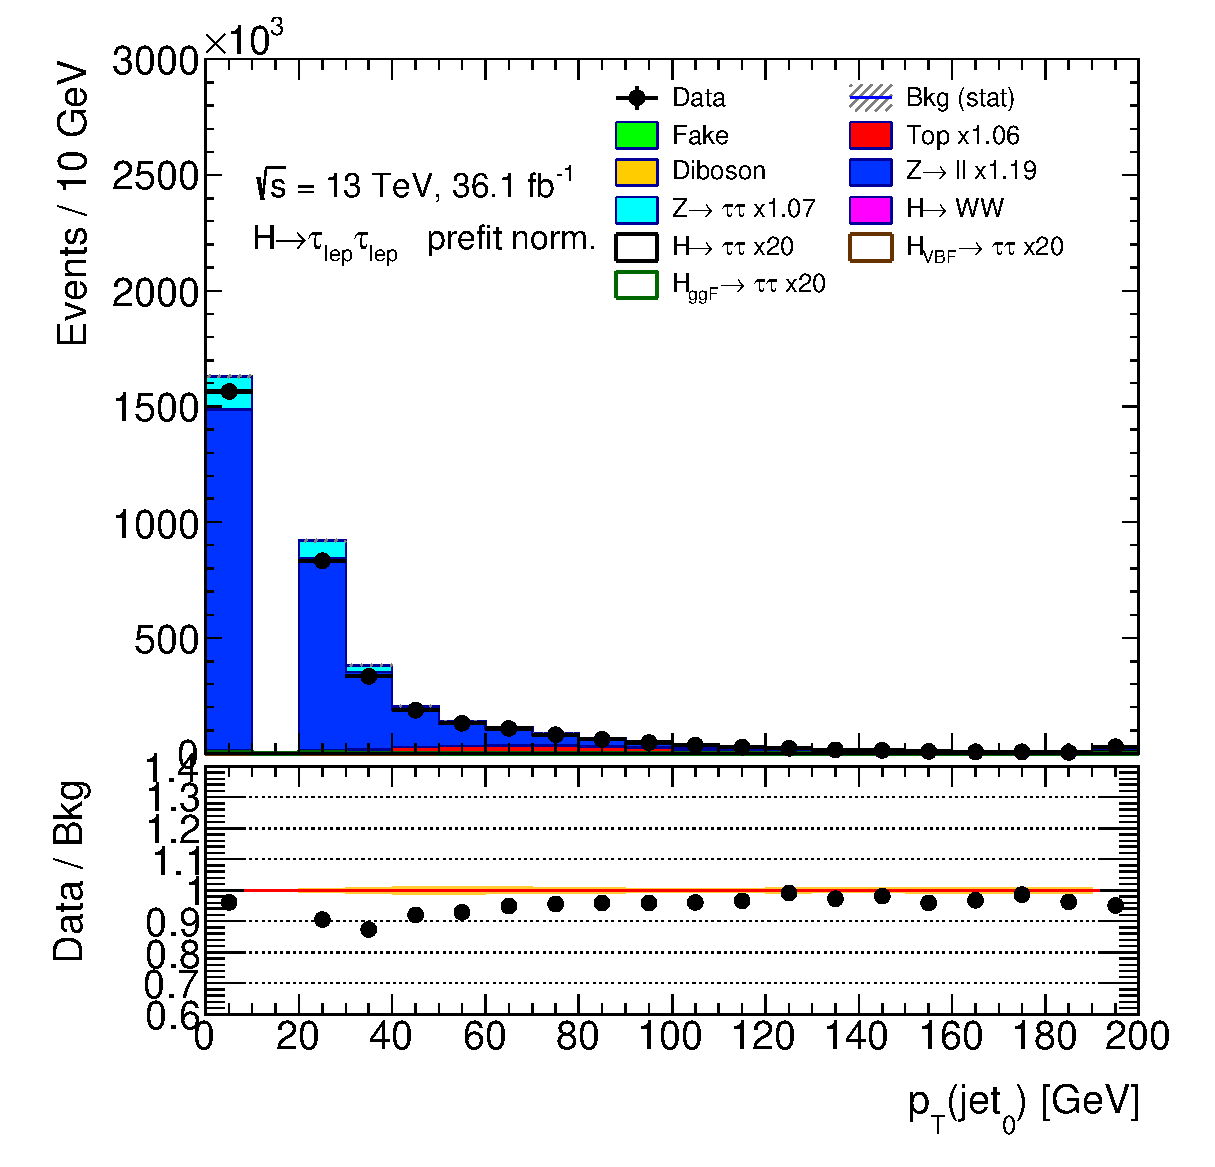
\includegraphics[width=0.45\textwidth]{./plots/event_selection/ll-CutMVis-JetPt0-lin.eps}
    \caption{Distribution of $\pt^{\text{jet}_1}$ after Cut~10.
             Normalization factors are applied on the top-quark, $\Zll$, and $\Ztautau$ background.
             The signal is scaled by a factor of 20.
             Only statistical uncertainties are included in the error band.}\label{fig:event_selection:cutflow:jetlead}
\end{figure}

\begin{figure}[htb]
    \centering
    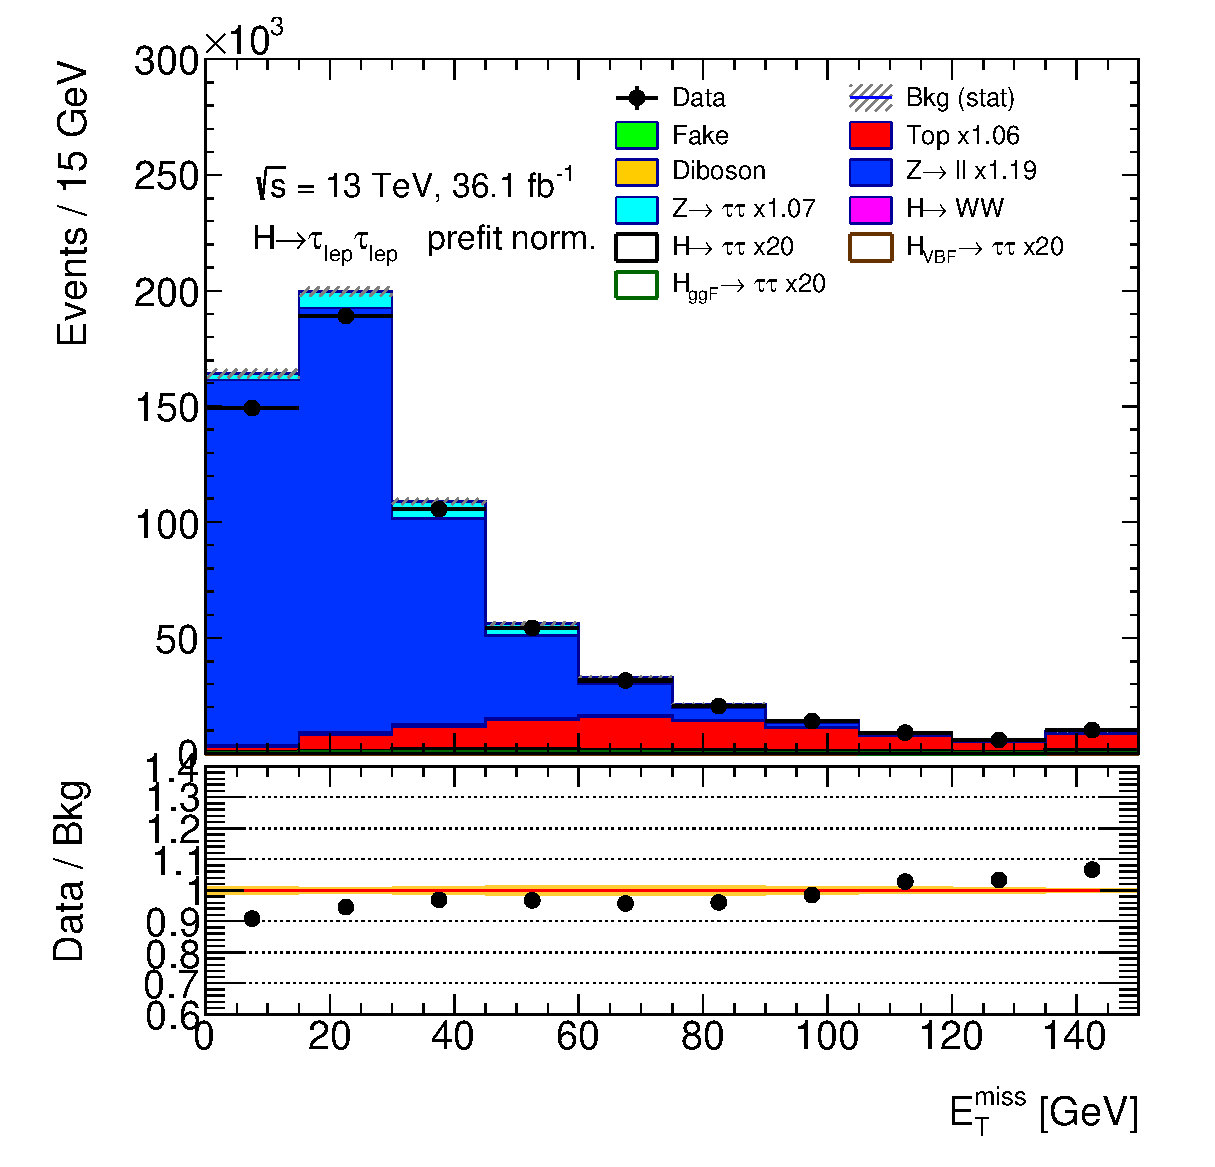
\includegraphics[width=0.45\textwidth]{./plots/event_selection/eemm-CutJet0Pt-MET-lin.eps}
    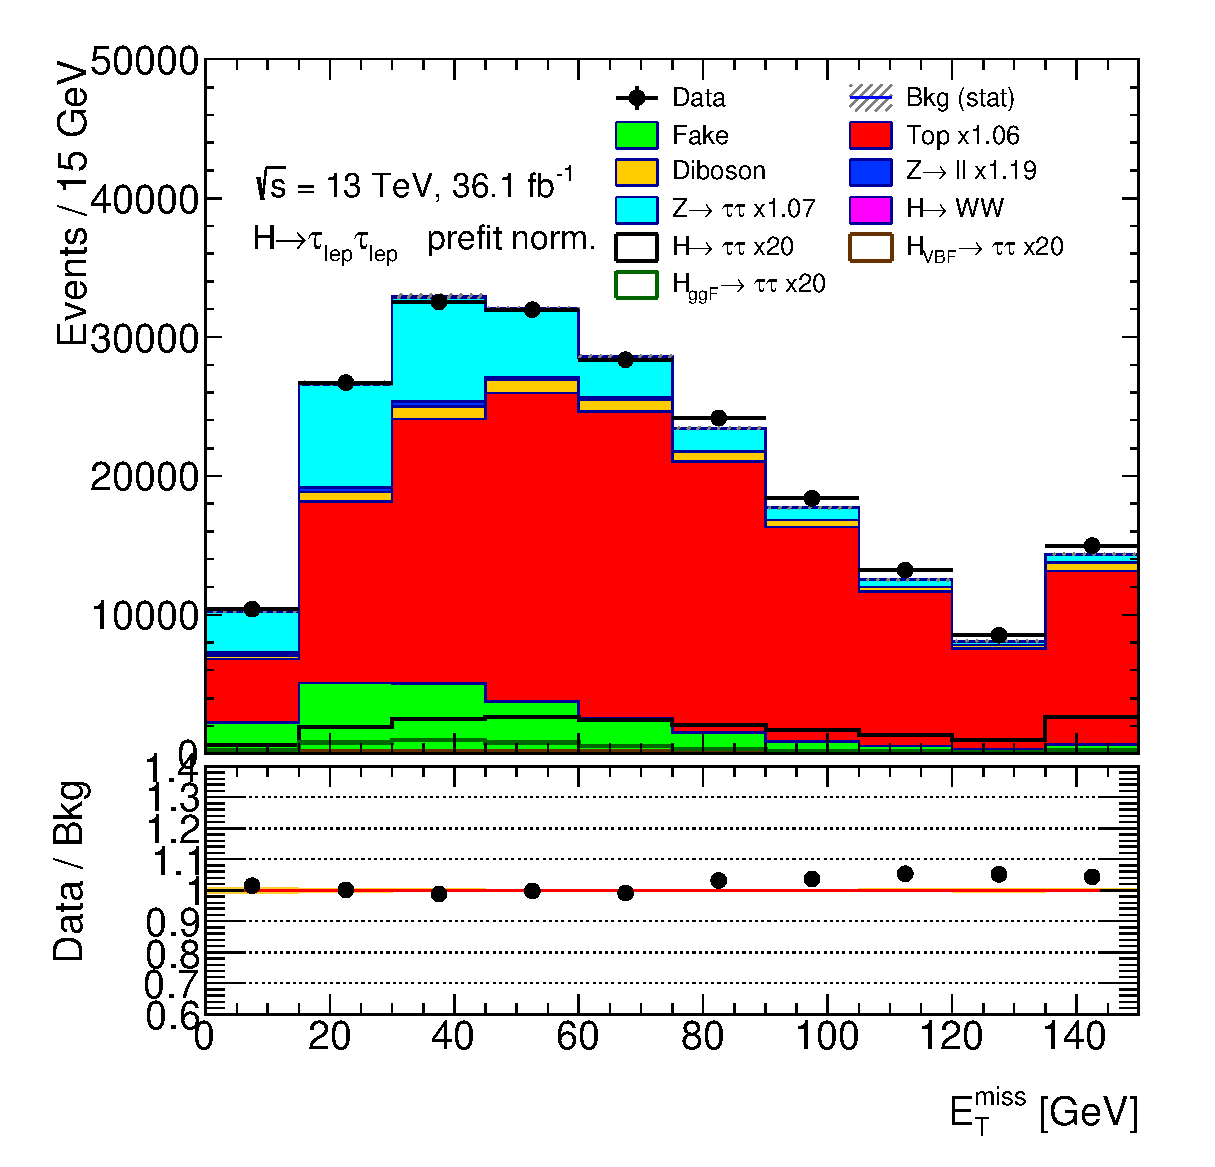
\includegraphics[width=0.45\textwidth]{./plots/event_selection/emme-CutJet0Pt-MET-lin.eps}
    \caption{Distribution of $\etmiss$ after Cut~11 for SF (left) and DF (right) events.
             Normalization factors are applied on the top-quark, $\Zll$, and $\Ztautau$ background.
             The signal is scaled by a factor of 20.
             Only statistical uncertainties are included in the error band.}\label{fig:event_selection:cutflow:met}
\end{figure}

\begin{figure}[htb]
    \centering
    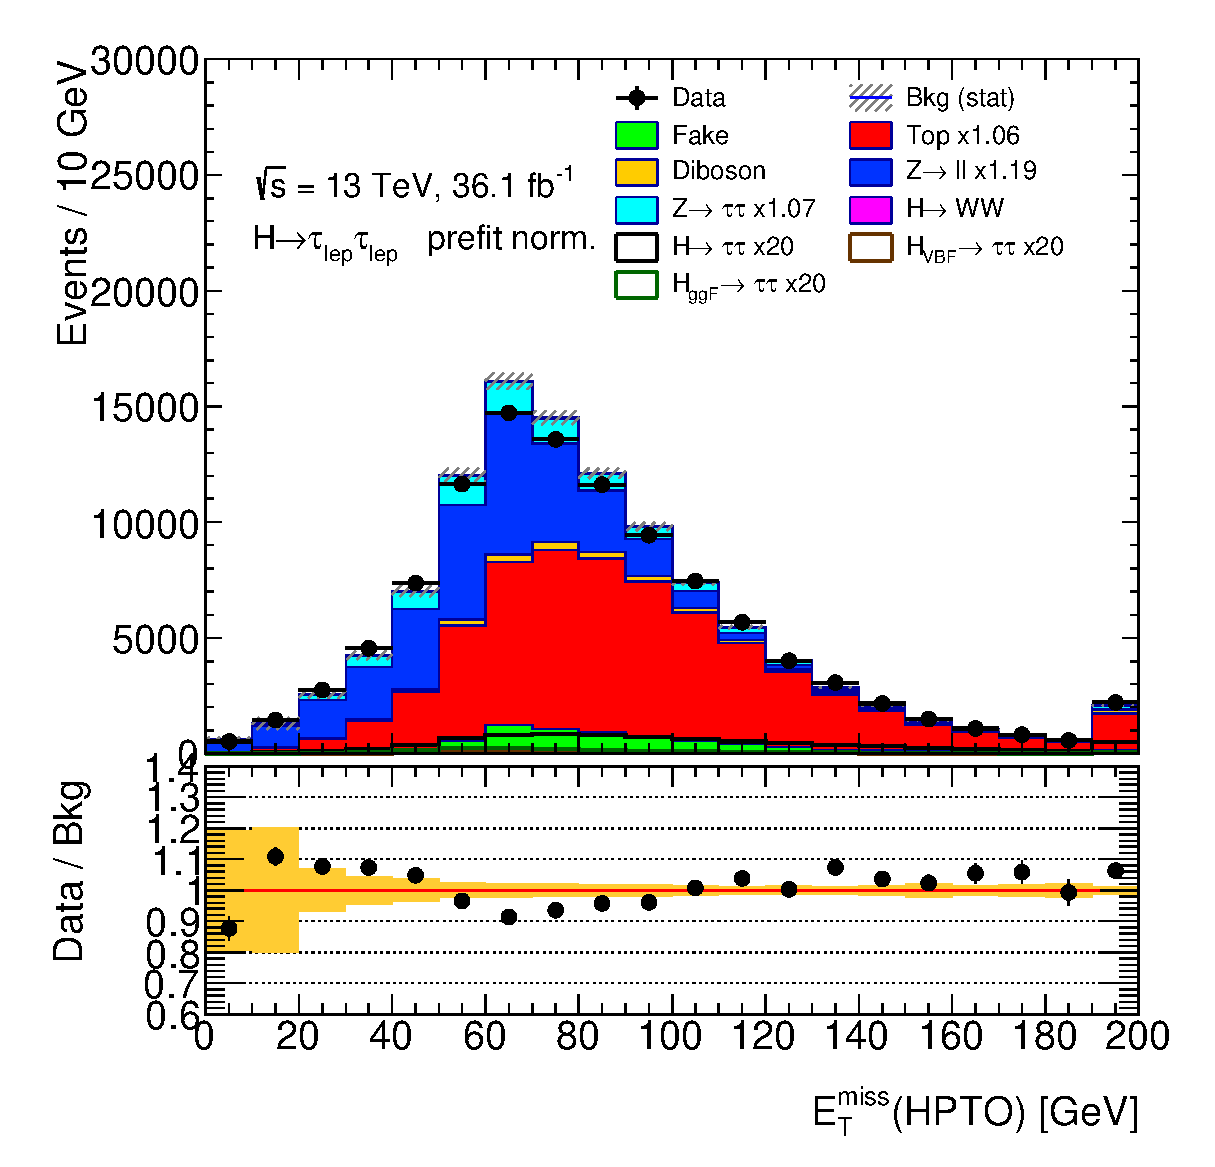
\includegraphics[width=0.45\textwidth]{./plots/event_selection/eemm-CutMET-METhpto-lin.eps}
    \caption{Distribution of $\etmisshpto$ after Cut~12.
             Normalization factors are applied on the top-quark, $\Zll$, and $\Ztautau$ background.
             The signal is scaled by a factor of 20.
             Only statistical uncertainties are included in the error band.}\label{fig:event_selection:cutflow:hpto}
\end{figure}

\begin{figure}[htb]
    \centering
    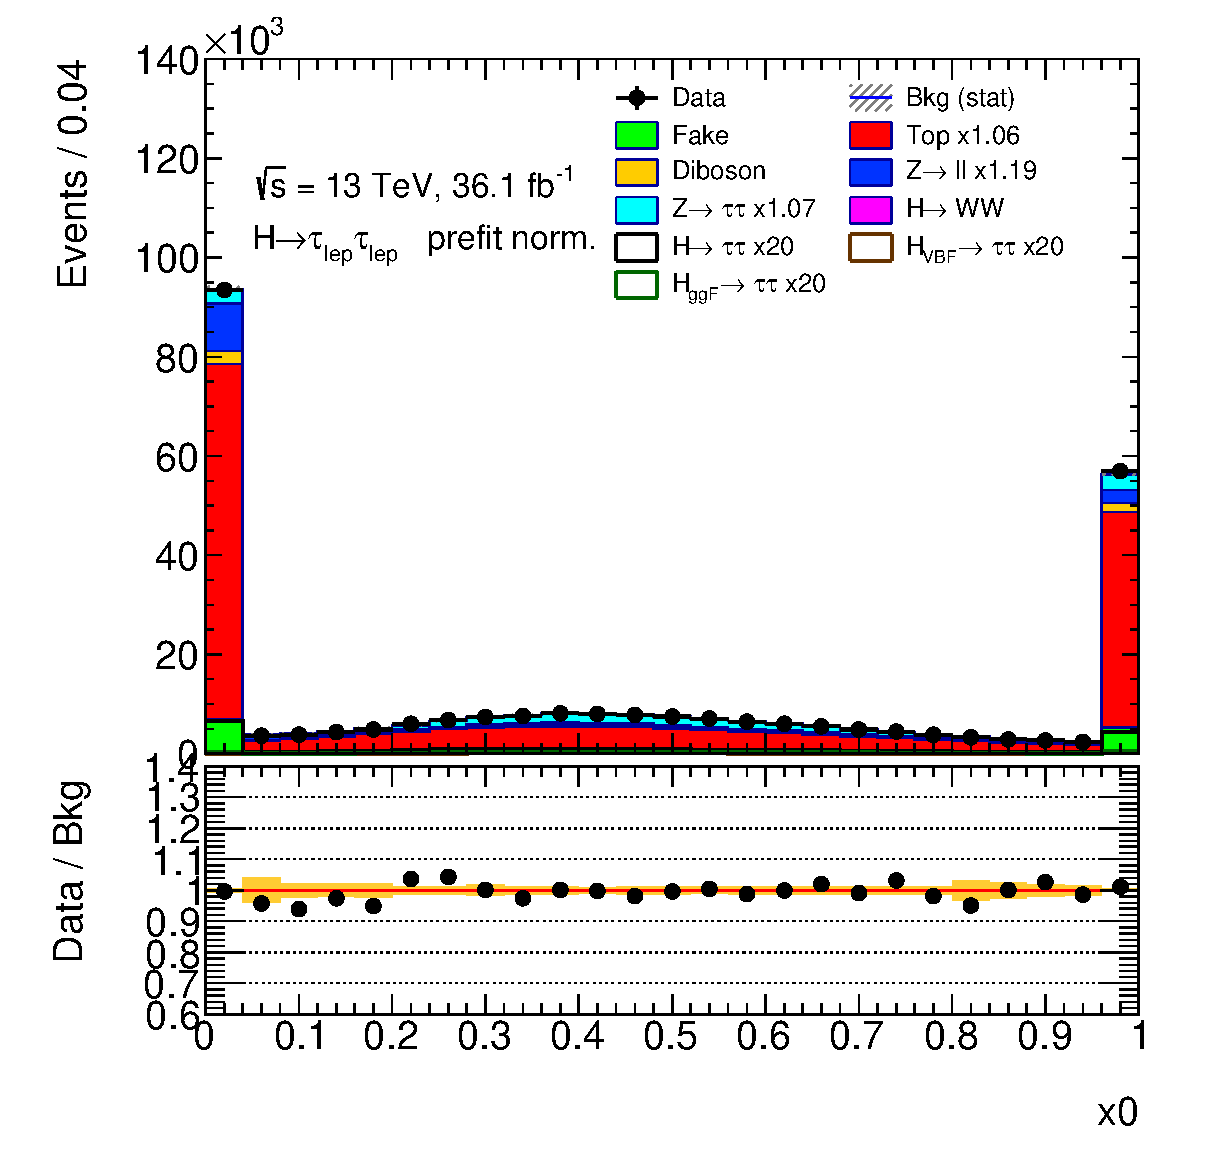
\includegraphics[width=0.45\textwidth]{./plots/event_selection/ll-CutHPTO-x0-lin.eps}
    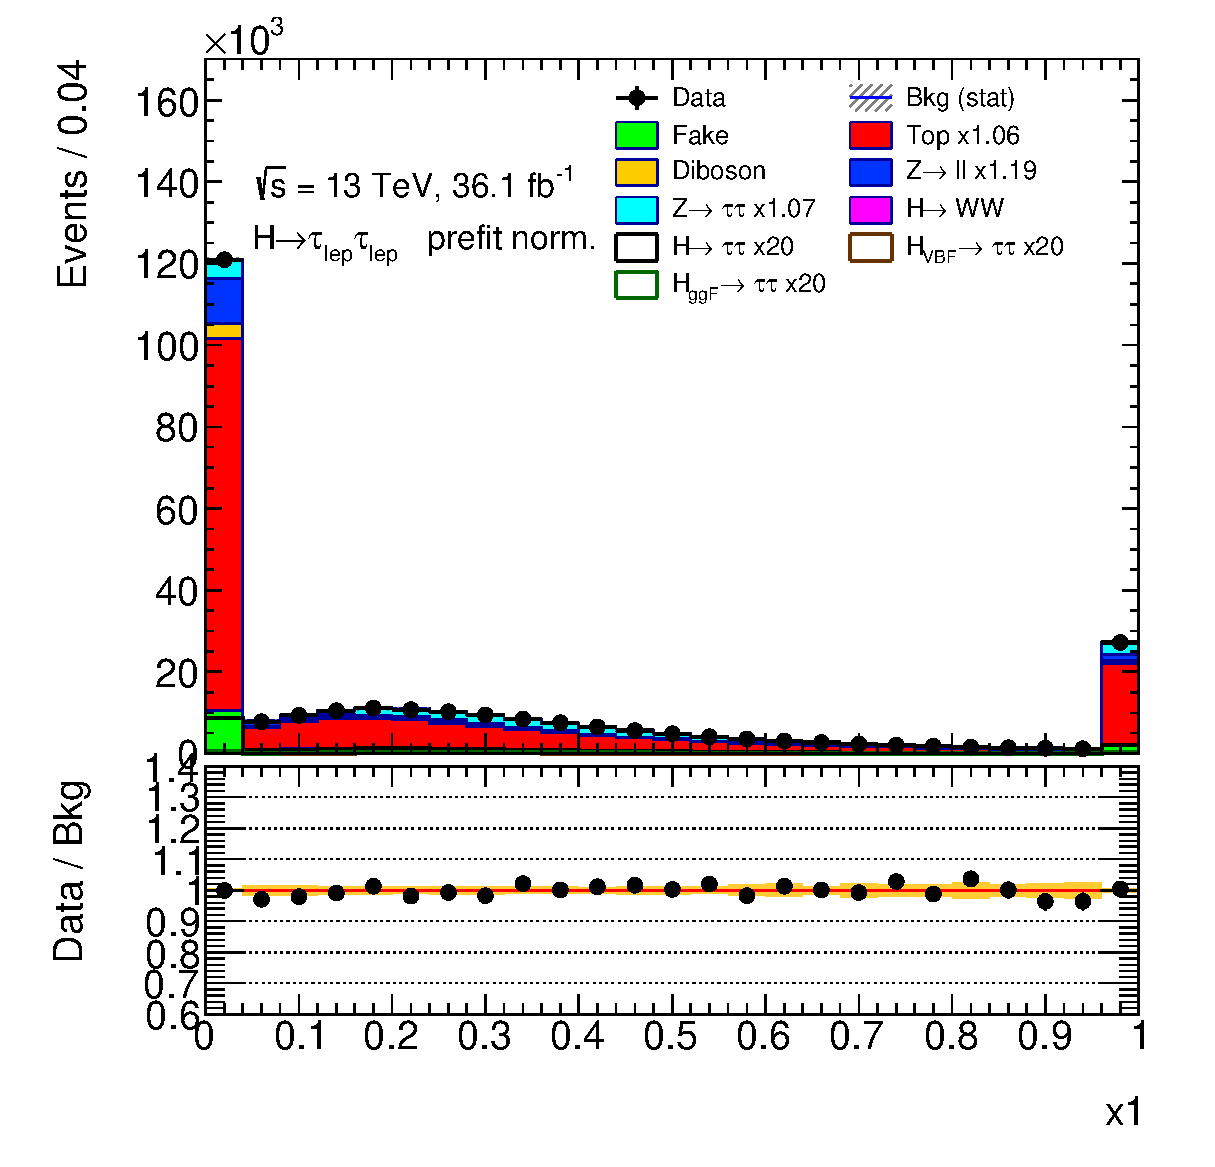
\includegraphics[width=0.45\textwidth]{./plots/event_selection/ll-CutHPTO-x1-lin.eps}
    \caption{Distributions of $x_1$ (left) and $x_2$ (right) after Cut~13.
             Normalization factors are applied on the top-quark, $\Zll$, and $\Ztautau$ background.
             The signal is scaled by a factor of 20.
             Only statistical uncertainties are included in the error band.}\label{fig:event_selection:cutflow:x}
\end{figure}

\begin{figure}[htb]
    \centering
    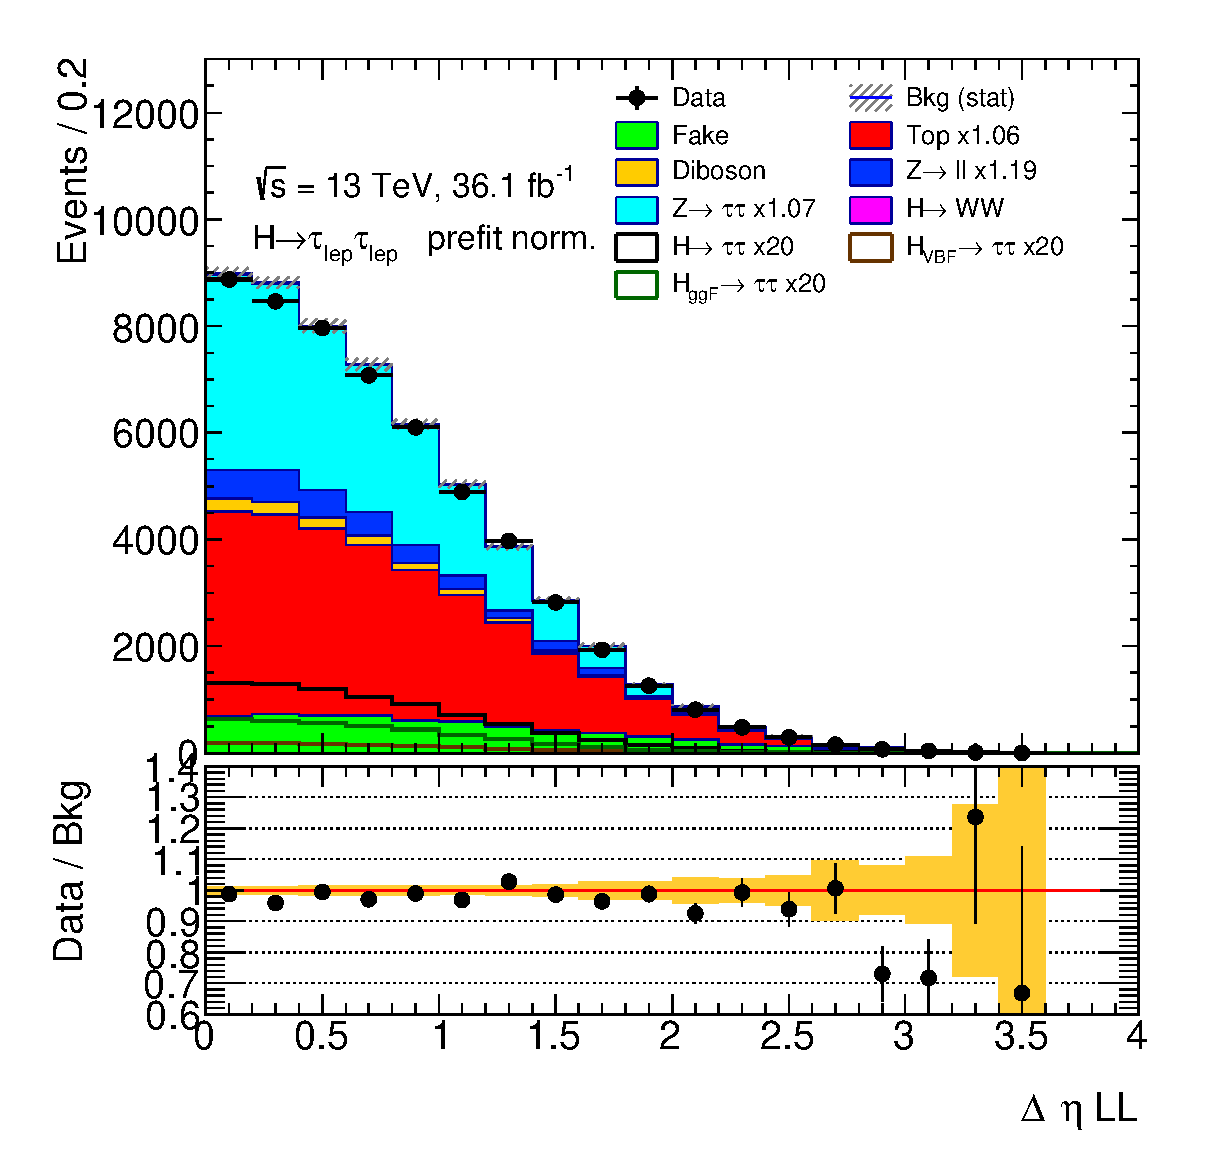
\includegraphics[width=0.45\textwidth]{./plots/event_selection/ll-CutX-DeltaEtaLL-lin.eps}
    \caption{Distribution of $\absdetall$ after Cut~14.
             Normalization factors are applied on the top-quark, $\Zll$, and $\Ztautau$ background.
             The signal is scaled by a factor of 20.
             Only statistical uncertainties are included in the error band.}\label{fig:event_selection:cutflow:detall}
\end{figure}

\begin{figure}[htb]
    \centering
    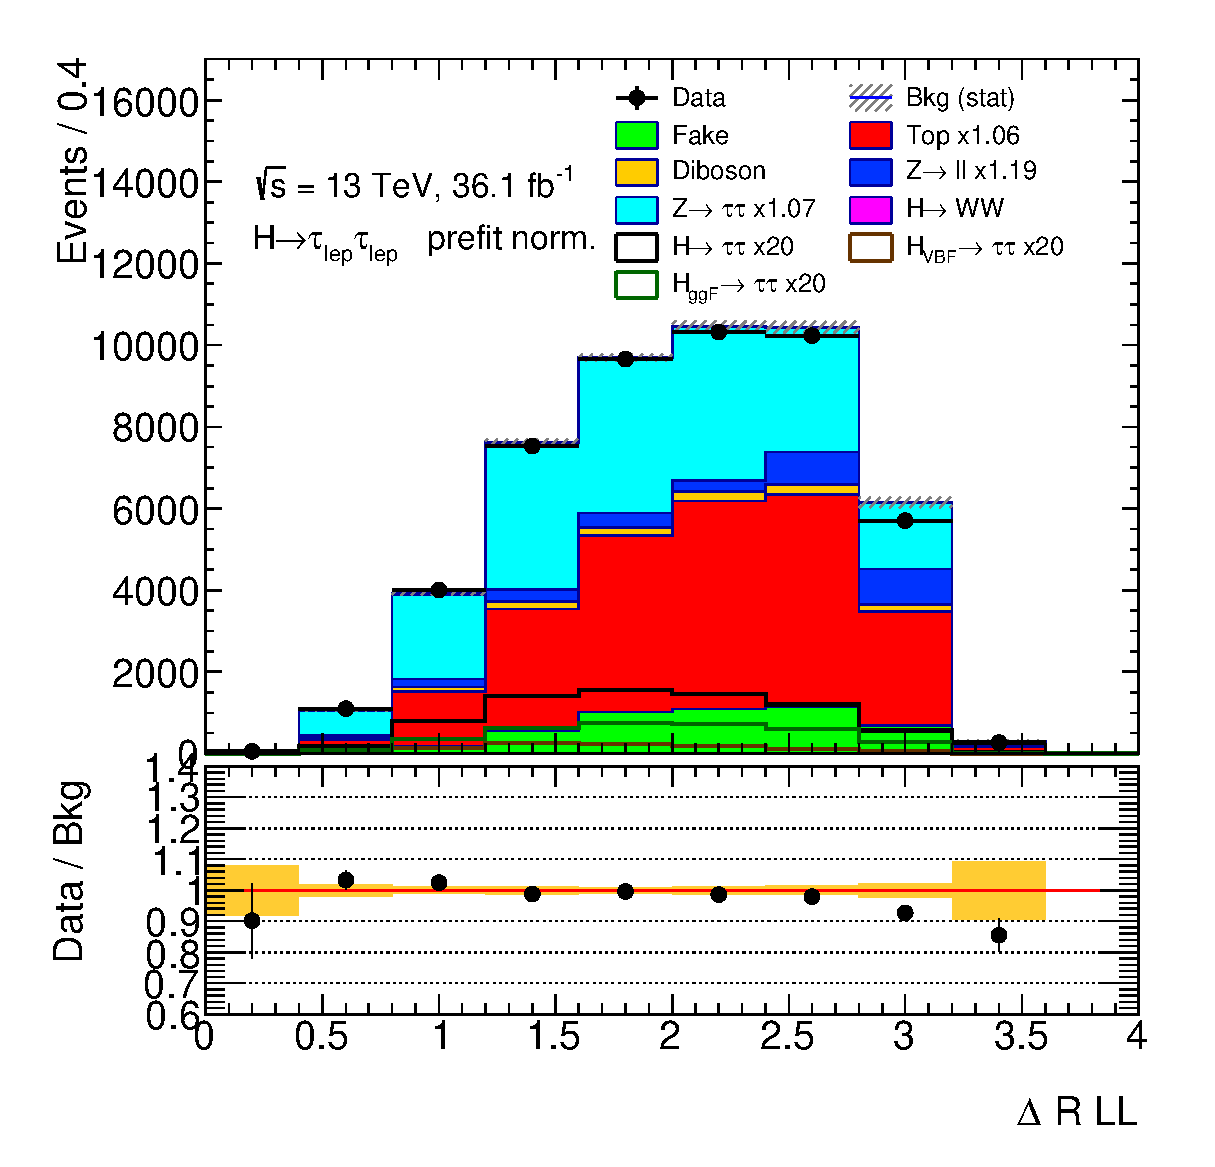
\includegraphics[width=0.45\textwidth]{./plots/event_selection/ll-CutDEtaLL-DeltaRLL-lin.eps}
    \caption{Distribution of $\drll$ after Cut~15.
             Normalization factors are applied on the top-quark, $\Zll$, and $\Ztautau$ background.
             The signal is scaled by a factor of 20.
             Only statistical uncertainties are included in the error band.}\label{fig:event_selection:cutflow:drll}
\end{figure}

\begin{figure}[htb]
    \centering
    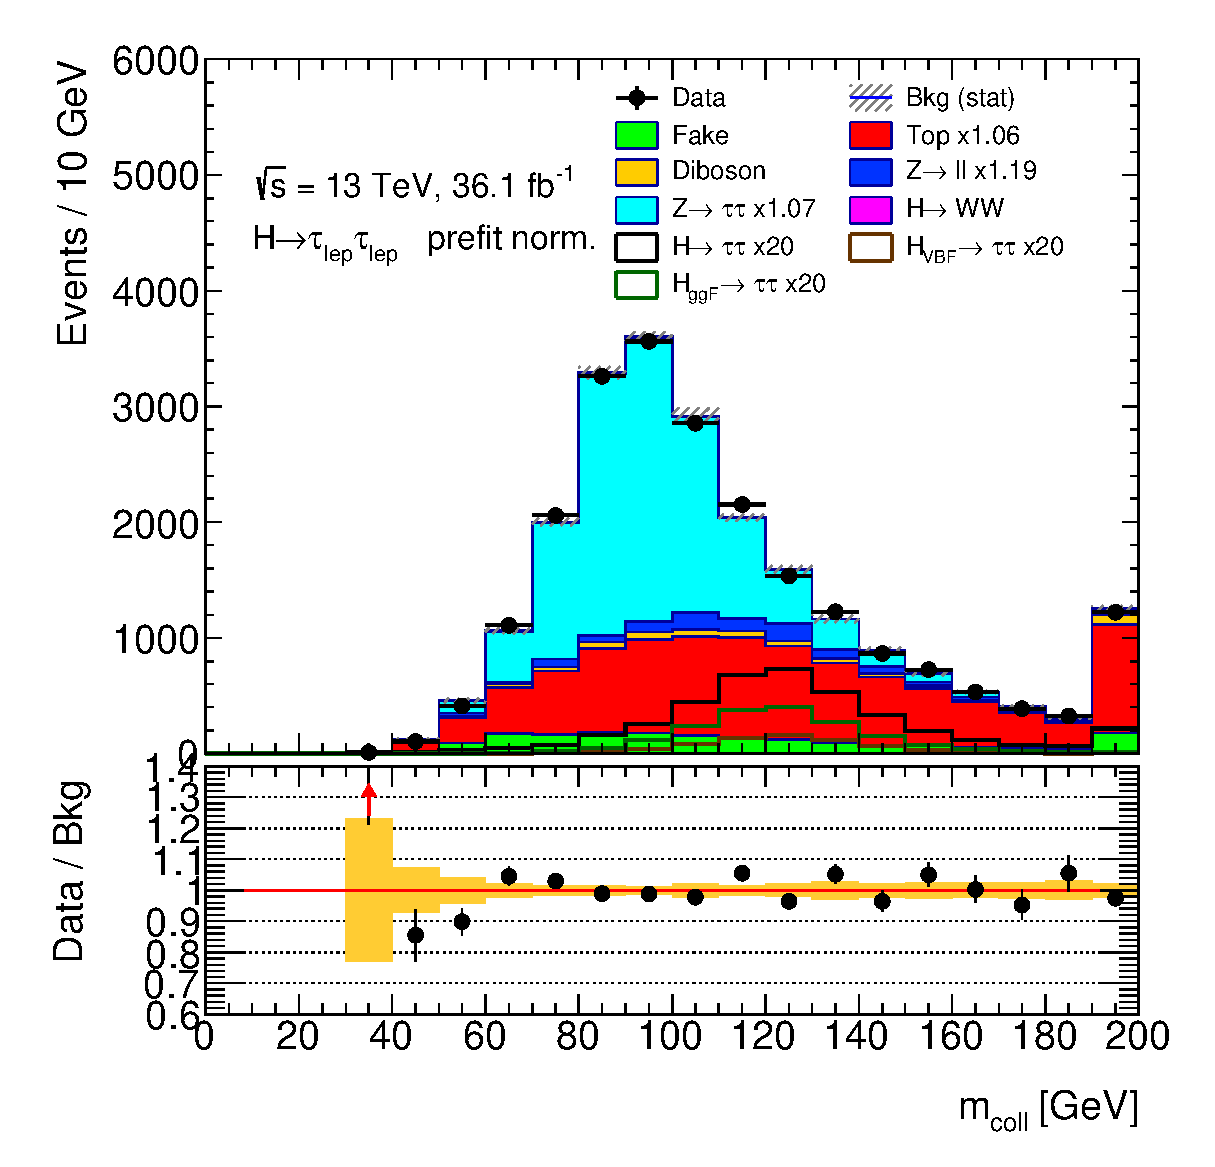
\includegraphics[width=0.45\textwidth]{./plots/event_selection/ll-CutDRLL-mcoll-lin.eps}
    \caption{Distribution of $\mcoll$ after Cut~16.
             Normalization factors are applied on the top-quark, $\Zll$, and $\Ztautau$ background.
             The signal is scaled by a factor of 20.
             Only statistical uncertainties are included in the error band.}\label{fig:event_selection:cutflow:mcoll}
\end{figure}


\section{Categorization}\label{sec:event_selection:categorization}

Since the goal of this analysis is to measure the coupling strength of the Higgs boson
in different production modes, dedicated categories for the VBF and gluon--gluon fusion production mode
are defined by exploiting production-mode specific event topologies.
They are referred to as the \emph{VBF} and \emph{boosted category}, respectively.

\subsection{VBF category}\label{sub:event_selection:vbf}

In the VBF production mode two vector bosons are used to produce the Higgs boson.
The vector bosons originate from two partons, which produce two jets with high transverse momentum
in the forward region of the detector.
The following cuts are applied to select this topology:\todo{Add plots with variables before they are cut on.}
\begin{description}[style=nextline,leftmargin=1cm]
    \item[(1V) Subleading jet momentum]
        A second jet is required with at least $\pt > \unit[30]{GeV}$.
    \item[(2V) Opposite hemispheres]
        The two leading jets need to occupy different hemispheres of the detector due to the VBF topology.
        This can be achieved by applying the $\eta_{\text{jet}_1} \cdot \eta_{\text{jet}_2} < 0$ requirement.
    \item[(3V) Angular separation of two leading jets]
        The separation in $\eta$ between the two VBF jets is expected to be large.
        Therefore, a cut of $\absdetajj > 3$ is applied.
    \item[(4V) Lepton candidate centrality]
        The $\eta$ of the selected leptons must lie in between the two jets.
    \item[(5V) Invariant mass of the dijet system]
        The dijet system is required to have an invariant mass of $\mjj > \unit[400]{GeV}$.
\end{description}
Furthermore, the VBF category is split into a \emph{high} and \emph{low} VBF category,
with requirements on the transverse momentum of the di-$\tau$ system, $\pt^{\tau\tau} > \unit[100]{GeV}$ and $\pt^{\tau\tau} < \unit[100]{GeV}$, respectively.
The transverse momentum of the di-$\tau$ system is calculated from the transverse momenta of the visible decay products of the
$\tau$-leptons and the missing transverse energy.
This helps to increase the sensitivity, provided that the statistics in the sub-categories are still high enough.

The distributions of $\mmc$ in the inclusive, high, and low VBF category is shown in \cref{fig:event_selection:vbf:mmc}.\todo{Include systematic uncertainties}

\begin{figure}[htb]
    \centering
    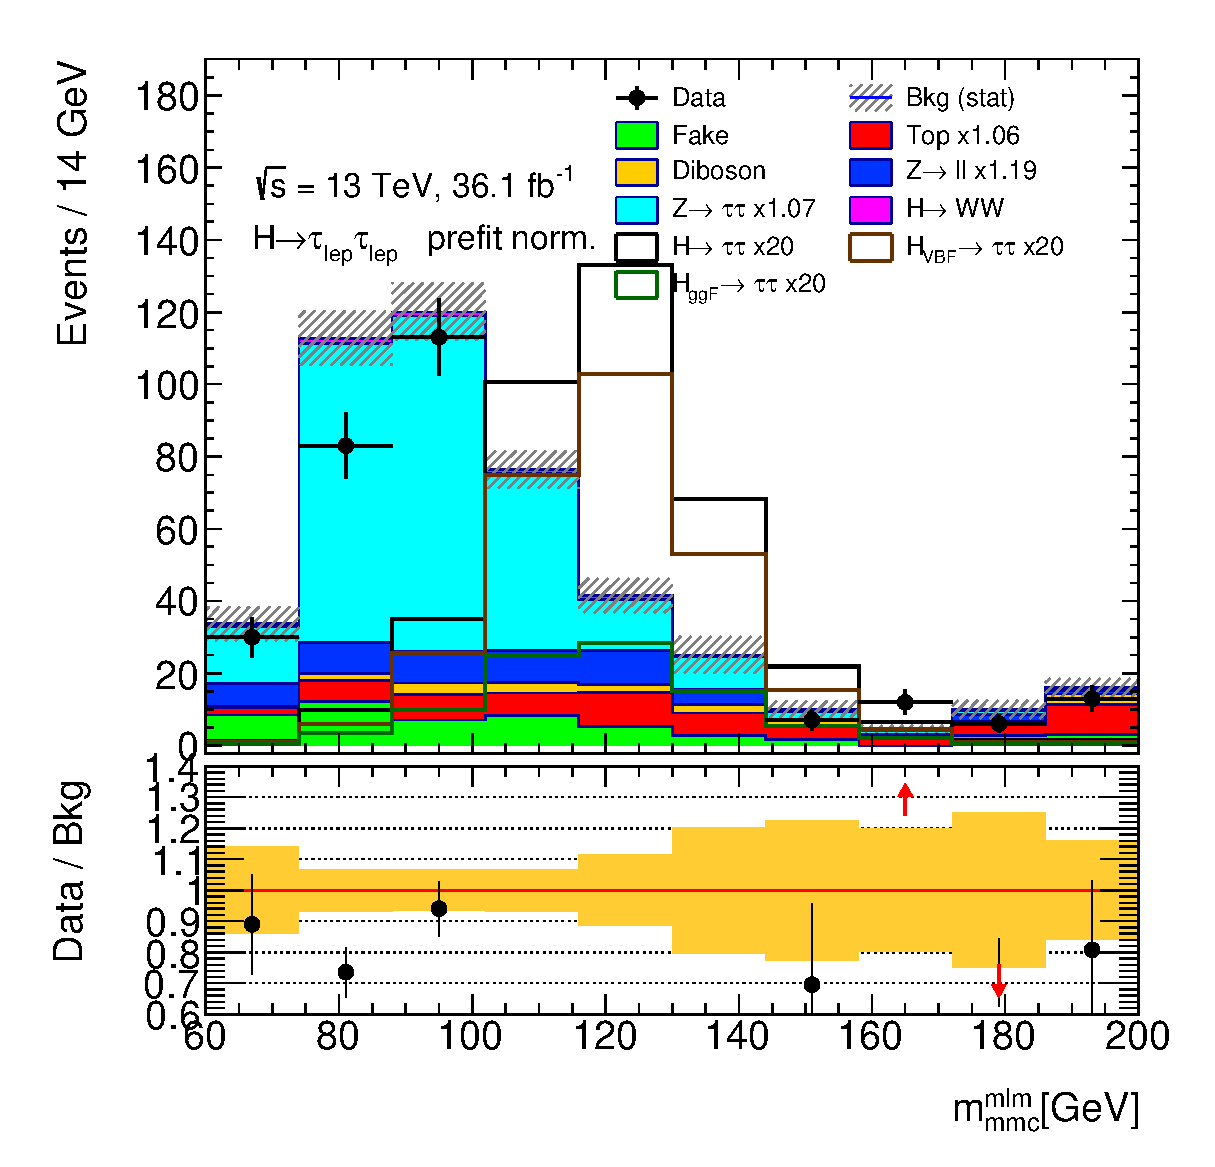
\includegraphics[width=0.3\textwidth]{./plots/event_selection/ll-CutVBFCat-dilep_mmc_mlm_m_vbf-lin.eps}
    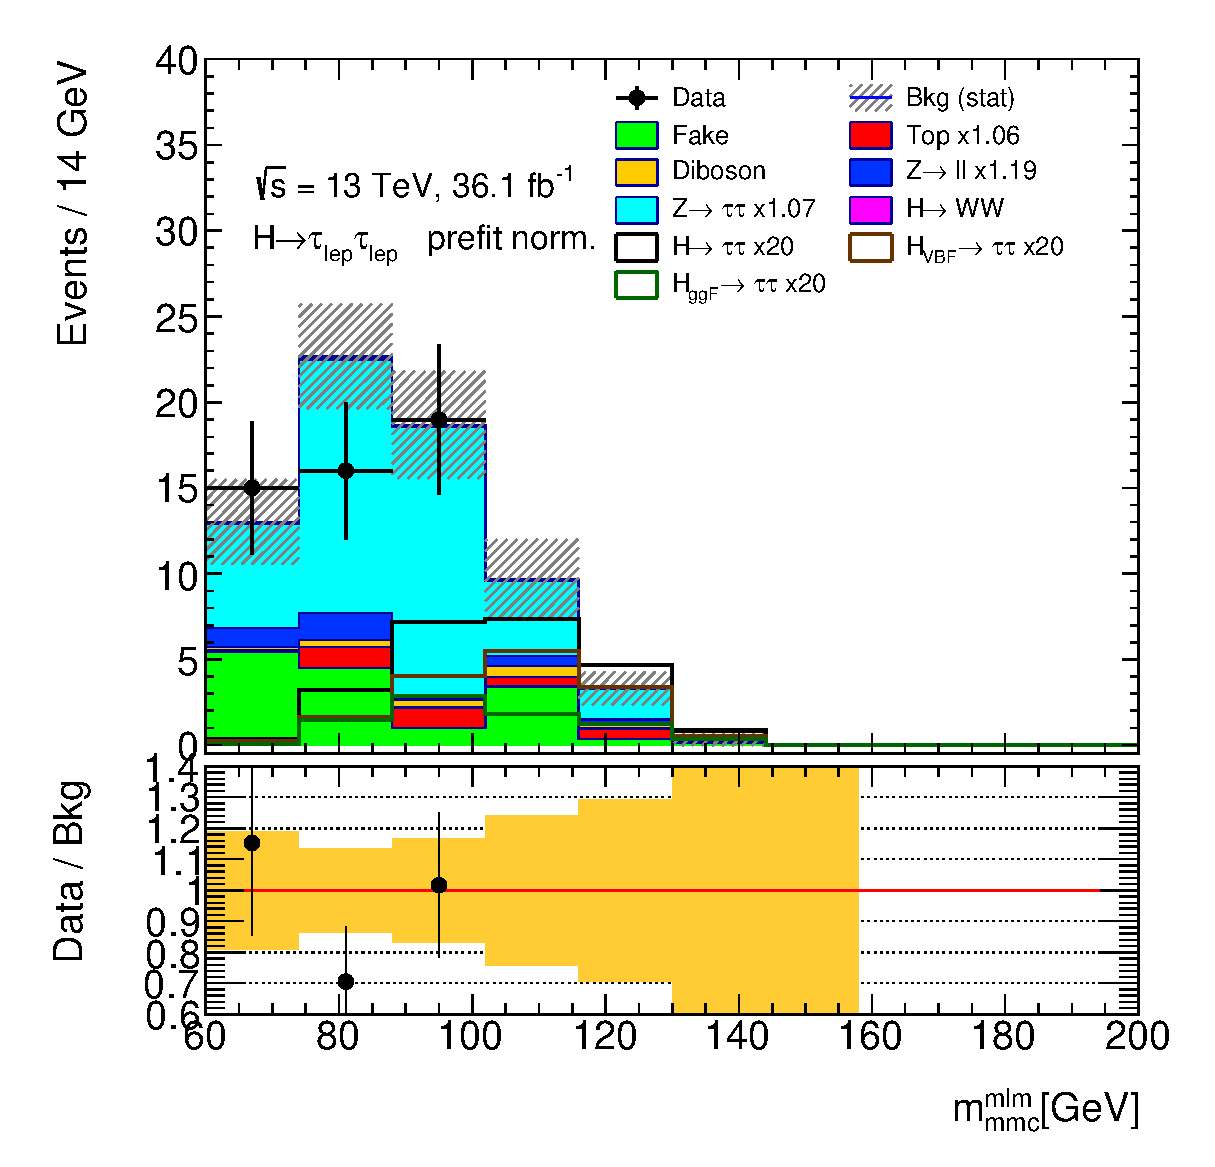
\includegraphics[width=0.3\textwidth]{./plots/event_selection/ll-CutVBFCatA-dilep_mmc_mlm_m_vbf-lin.eps}
    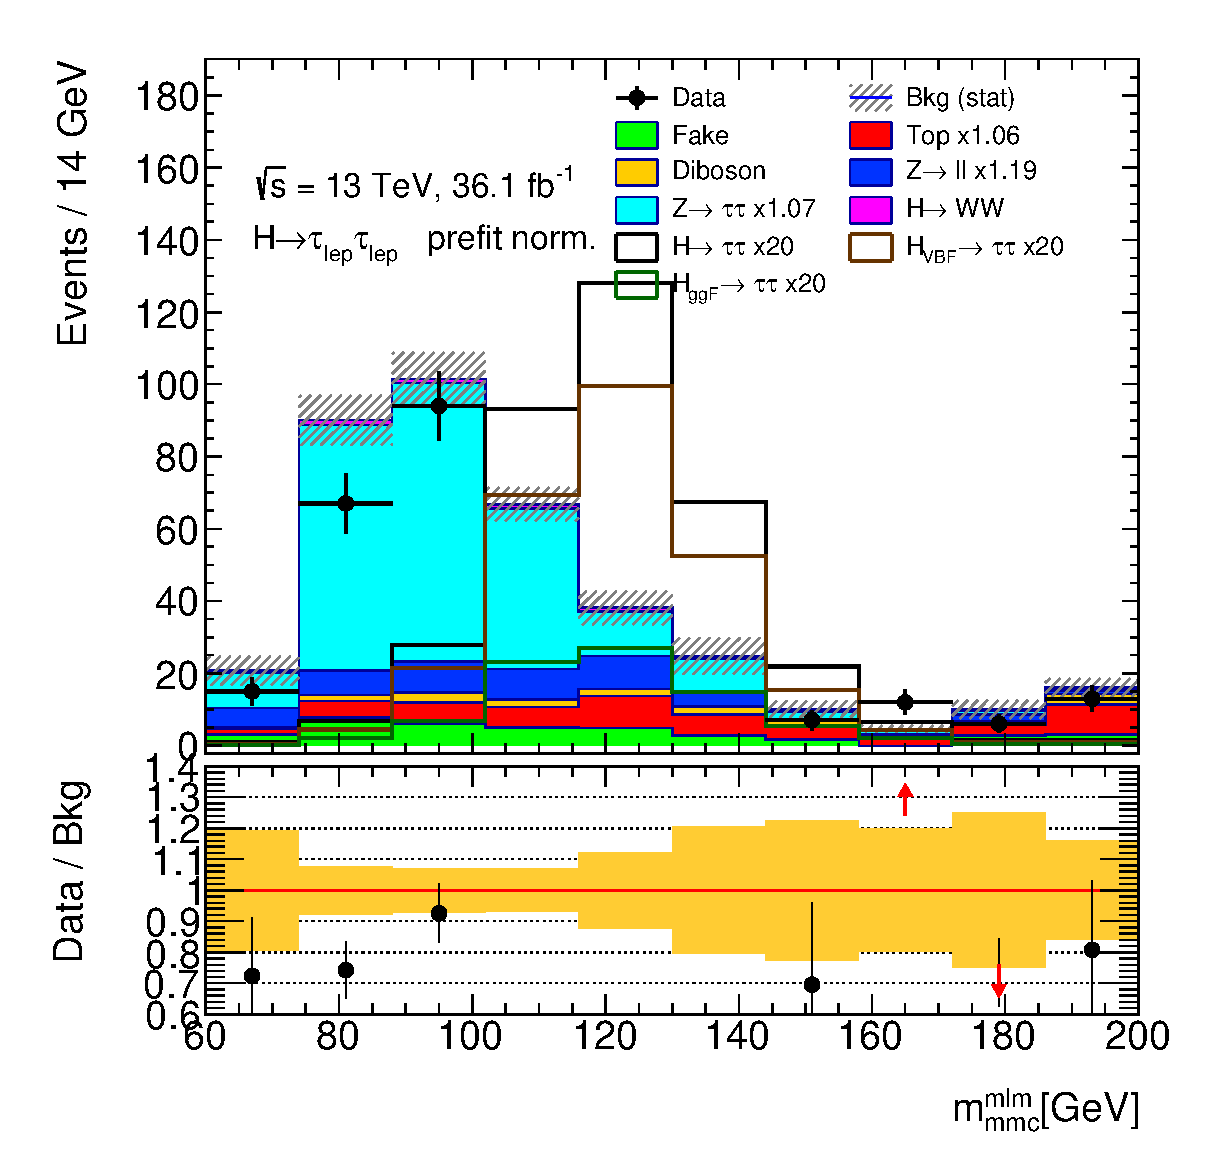
\includegraphics[width=0.3\textwidth]{./plots/event_selection/ll-CutVBFCatB-dilep_mmc_mlm_m_vbf-lin.eps}
    \caption{Distributions of the output of the missing mass calculator algorithm, $\mmc$, in the inclusive (left),
             low (middle), and high (right) VBF category.
             Normalization factors are applied on the top-quark, $\Zll$, and $\Ztautau$ background.
             The signal is scaled by a factor of 20.
             The error band includes statistic and systematic uncertainties.}\label{fig:event_selection:vbf:mmc}
\end{figure}

\subsection{Boosted category}\label{sub:event_selection:boosted}

In contrast to the VBF production mode, the gluon--gluon fusion production mode has no outgoing partons at tree-level.\todo{Ref feynman graph in theory chapter}
However, higher order QCD corrections can produce a recoil jet, which leads to a high transverse momentum of the Higgs boson.
This helps to suppress the irreducible $\Ztautau$ background.
The selection criteria for the boosted category are as follows:\todo{Add plots with variables before they are cut on.}
\begin{description}[style=nextline,leftmargin=1cm]
    \item[(1B) Veto on VBF selection]
        The events have to pass the preselection, but not the VBF selection.
    \item[(2B) Higgs boson transverse momentum]
        The transverse momentum of the di-$\tau$ system is required to be $\pt^{\tau\tau} > \unit[100]{GeV}$.
\end{description}
Similar to the VBF category, also the boosted category is divided into two sub-categories.
All events which pass the requirements $\pt^{\tau\tau} > \unit[140]{GeV}$ and $\drll < 1.5$ are sorted
into the \emph{high-boosted} category. All other events which do not pass these criteria are filled in the
\emph{low-boosted} category.

\cref{fig:event_selection:boosted:mmc} shows the distributions of $\mmc$ in the inclusive boosted, low-boosted, and high-boosted regions.
\todo{Include systematic uncertainties}

\begin{figure}[htb]
    \centering
    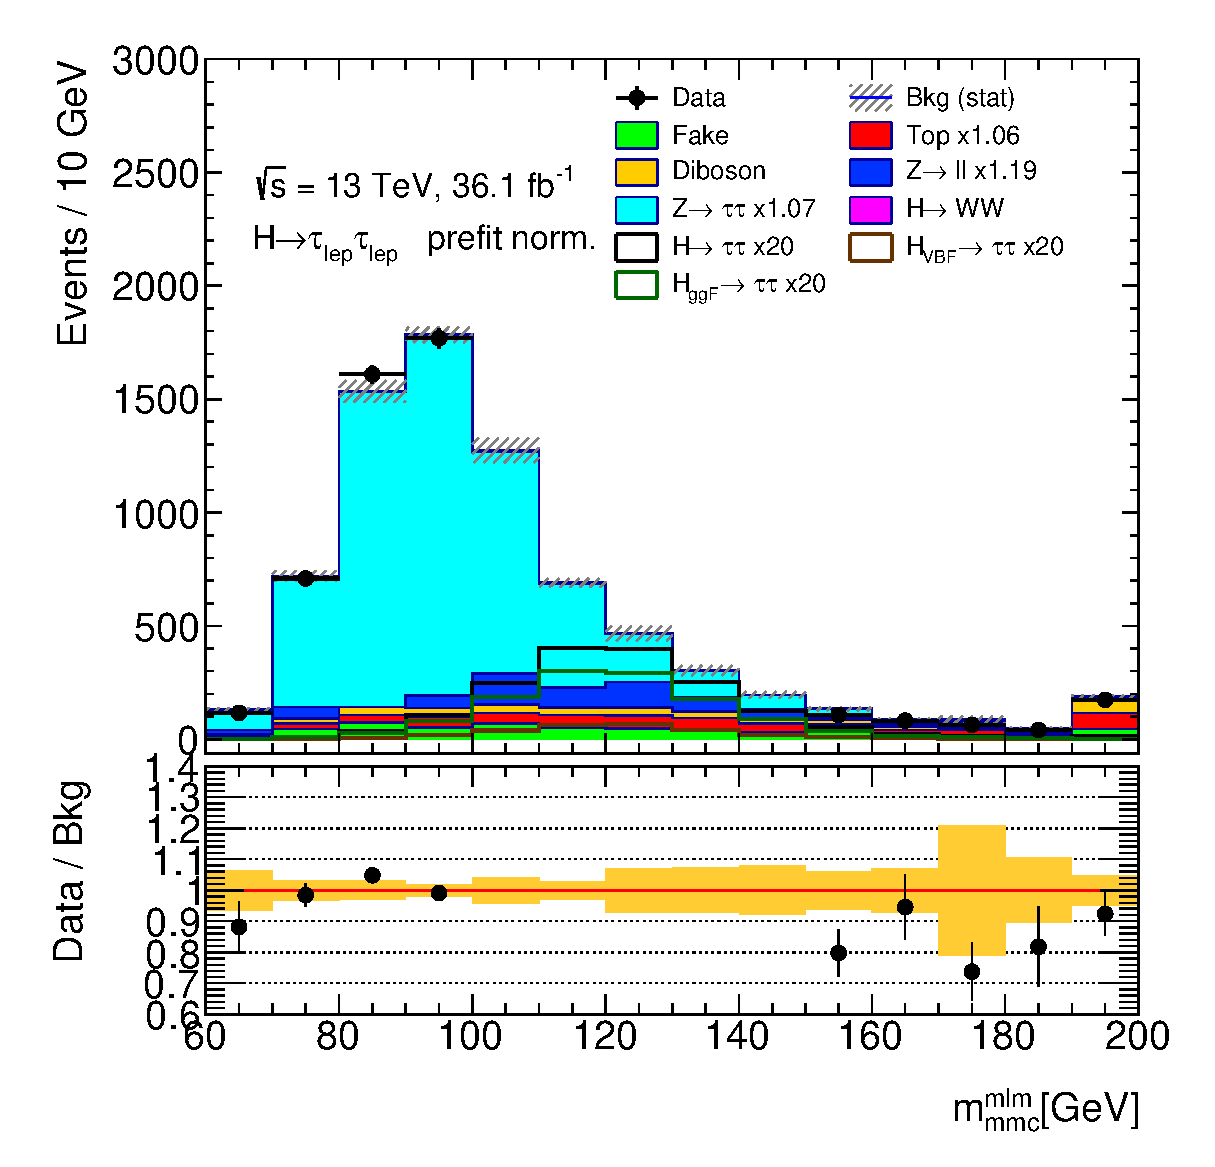
\includegraphics[width=0.3\textwidth]{./plots/event_selection/ll-CutBoostedCat-dilep_mmc_mlm_m-lin.eps}
    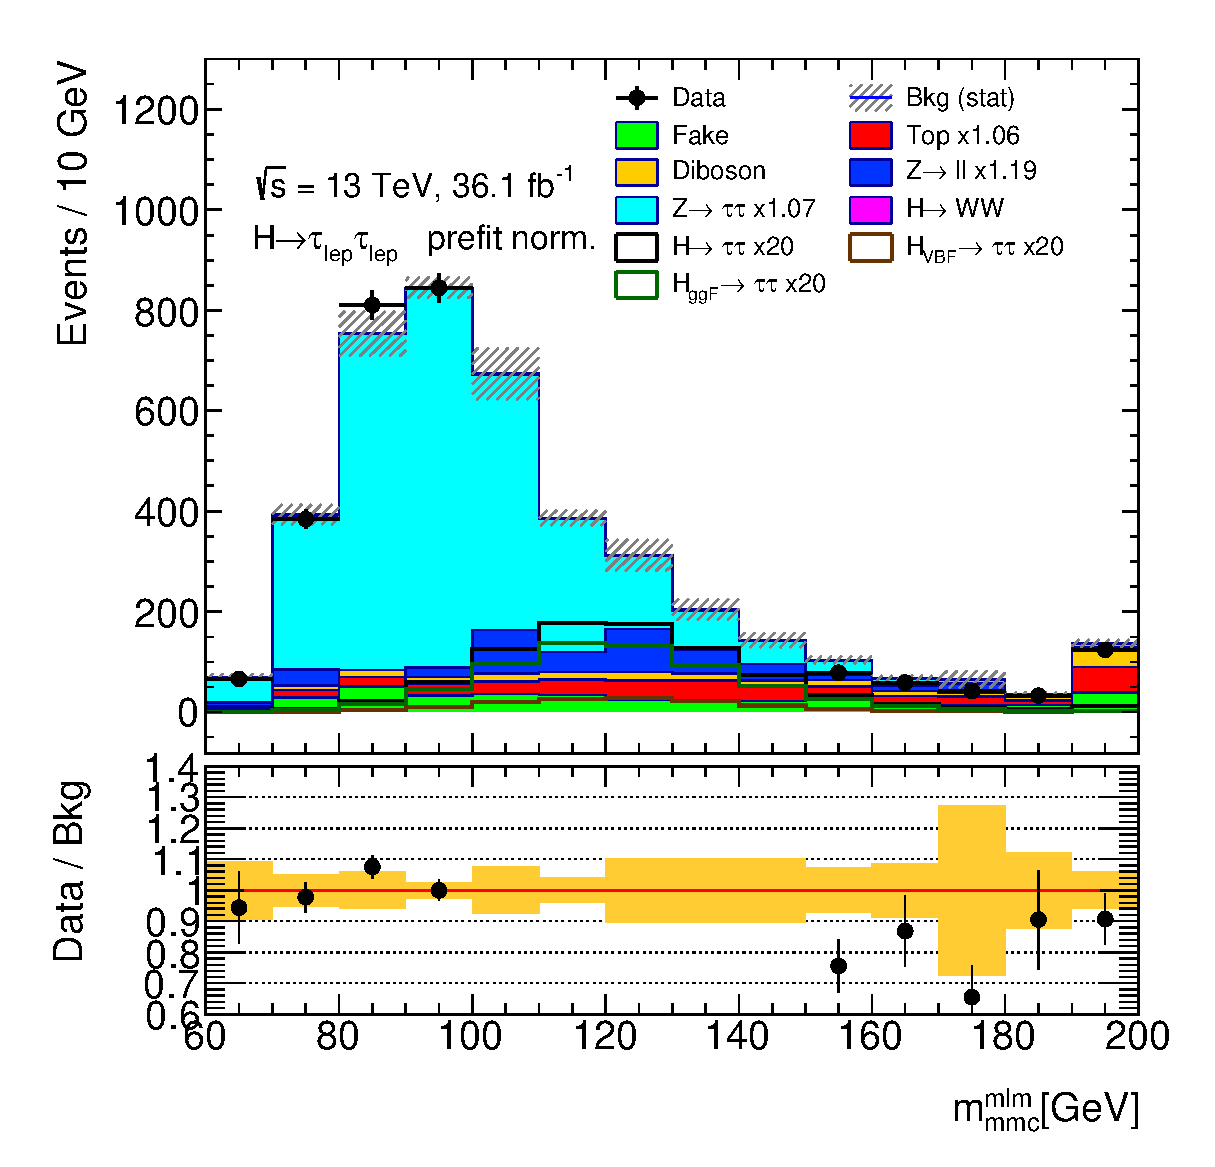
\includegraphics[width=0.3\textwidth]{./plots/event_selection/ll-CutBoostedCatA-dilep_mmc_mlm_m-lin.eps}
    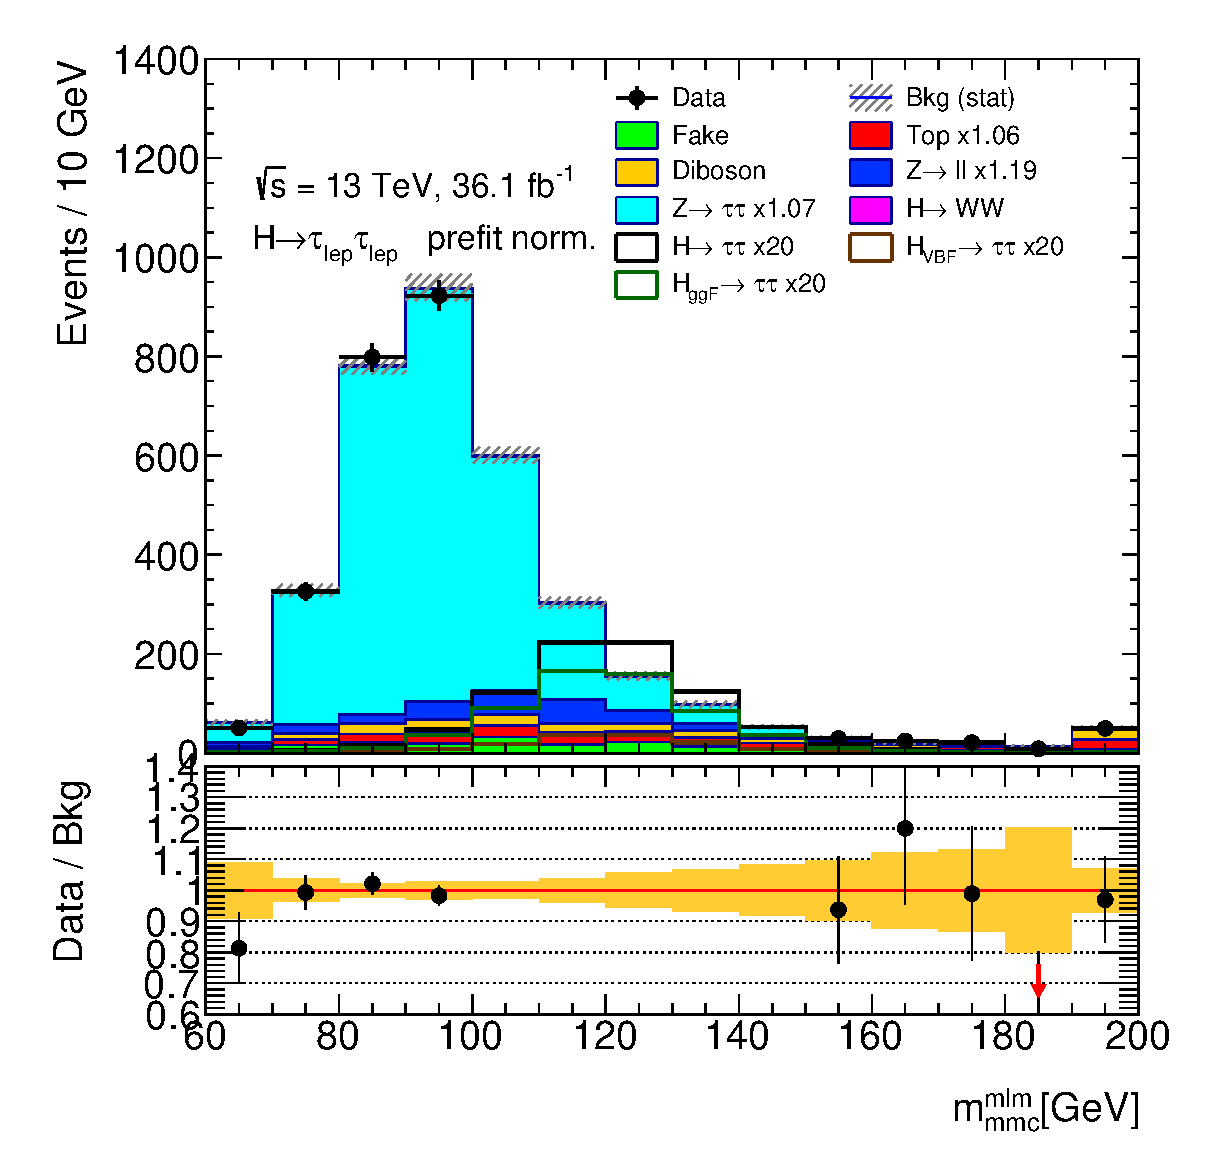
\includegraphics[width=0.3\textwidth]{./plots/event_selection/ll-CutBoostedCatB-dilep_mmc_mlm_m-lin.eps}
    \caption{Distributions of the output of the missing mass calculator algorithm, $\mmc$, in the inclusive boosted (left),
             low-boosted (middle), and high-boosted (right) boosted category.
             Normalization factors are applied on the top-quark, $\Zll$, and $\Ztautau$ background.
             The signal is scaled by a factor of 20.
             The error band includes statistic and systematic uncertainties.}\label{fig:event_selection:boosted:mmc}
\end{figure}

\section{Event yields}\label{sec:event_selection:yields}

\cref{tab:event_selection:yields} shows the event yields for the different signal and background processes after
the preselection and in the inclusive VBF and boosted categories.
\todo{Observations in event yields}
\todo{Fill out table}

\begin{table}[htpb]
    \centering
    \caption{Event yields for the different signal and background processes after the preselection
             and in the inclusive VBF and boosted categories with a combined 2016 and 2016 dataset of $\unit[36.1]{fb^{-1}}$.
             Normalization factors are applied on the top-quark, $\Zll$, and $\Ztautau$ background.
             Only statistical uncertainties are shown.}\label{tab:event_selection:yields}
    \begin{tabular}{lrrr}
        \toprule
        Process             & Preselection & VBF category & Boosted category \\ \midrule
        ggF $\Htt$          & & & \\
        VBF $\Htt$          & & & \\
        WH  $\Htt$          & & & \\
        ZH  $\Htt$          & & & \\
        ttH $\Htt$          & & & \\ \midrule
        Fakes               & & & \\
        Top                 & & & \\
        Diboson             & & & \\
        $\Zgammall$         & & & \\
        $\Zgammatt$         & & & \\
        $\HWW$              & & & \\ \midrule
        Total signal        & & & \\
        Total background    & & & \\ \midrule
        Data                & & & \\ \bottomrule
    \end{tabular}
\end{table}
